
%%%%%%%%%%%%%%%%%%%%%%%%%%%%%%%%%%%%%%%%%%%%%%%%%%%%%%%%%
\documentclass[inzynierska]{pwr_wmat_praca_dyplomowa}
\usepackage{graphicx}
\usepackage{ amssymb }
\usepackage{ dsfont }
\usepackage{amsmath}
\usepackage{algpseudocode}
\usepackage{indentfirst}
\graphicspath{{C:/Users/micha/Desktop/inzynier/NBA_Simulator/grafika/}} 
\usepackage{float}
\floatstyle{plaintop}
\restylefloat{table}

\autor{Michał Cerazy}
\tytul{Zastosowanie metod bootstrapowych do prognozowania wyników w zawodach sportowych} 
\tytulang{Application of bootstrap methods to the forecasting of sporting event results}
\opiekun{dr hab.\ inż.\ Krzysztof Burnecki}
\kierunekstudiow{Matematyka Stosowana}
\kierunekstudiowang{Applied Mathematics}
\specjalnosc{--} 
\specjalnoscang{--} 
\streszczenie{Praca dotyczy aktualnego problemu z matematyki stosowanej, a mianowicie stworzenia symulatora ligi NBA przy użyciu znanych technik matematycznych/statystycznych. Celem pracy było stworzenie symulatora rozgrywek w lidze NBA przy użyciu metod bootstrapowych. Wynikiem pracy jest oprogramowanie do symulacji rozgrywek w lidze NBA, wykonane przy pomocy języka Python, umożliwiające prognozowanie wyników w następnym roku. Otrzymane wyniki symulacji wskazują na małą skuteczność takiego podejścia.}
\streszczenieang{The main subject of the thesis concerns the recent problem from applied mathematics field --- creation of NBA league simulator using known mathematical/statistical techniques. The goal was to design a simulator based on bootstrap methods, with the result being Python language software capable of predicting outcome of a NBA season in the next year. Obtained simulation results imply low effectivness of this approach.}
\slowakluczowe{bootstrap, symulacje Monte Carlo, estymacja rozkładu, symulacja wyników koszykarskich}  
\slowakluczoweang{bootstrap, Monte Carlo simulations, fitting of distribution, simulation of basketball game outcomes}
%%%%%%%%%%%%%%%%%%%%%%%%%%%%%%%%%%%%%%%%%%%%%%%%%%%%%%%%%
% Definicje, lematy, twierdzenia, przykłady i wnioski
% Komendy wywołujące twierdzenia, definicje, itd., 
% czyli 'theorem', 'definition', 'corollary', itd., 
% można zmienić wedle uznania.
\theoremstyle{plain}
\newtheorem{theorem}{Twierdzenie}
\numberwithin{theorem}{chapter}
\newtheorem{lemma}[theorem]{Lemat} 
\newtheorem{corollary}[theorem]{Wniosek}
\newtheorem{fact}[theorem]{Fakt}
\theoremstyle{definition}
\numberwithin{theorem}{chapter}
\newtheorem{definition}[theorem]{Definicja} 
\newtheorem{algorytm}[theorem]{Algorytm}
\newtheorem{pseudokod}[theorem]{Pseudokod}
\newtheorem{example}[theorem]{Przykład}
\newtheorem{note}[theorem]{Uwaga}
%%%%%%%%%%%%%%%%%%%%%%%%%%%%%%%%%%%%%%%%%%%%%%%%%%%%%%%%%
\begin{document}
\frontmatter
\maketitle
\mainmatter
\tableofcontents
%\listoffigures
%\listoftables

{\backmatter \chapter{Wstęp}}
%We wstępie zapowiadamy, o czym będzie praca. Próbujemy zachęcić czytelnika do dalszej lektury, np. krótko informując, dlaczego wybraliśmy właśnie ten temat i co nas w nim zainteresowało.
Dzięki powszechnemu dostępowi do internetu i rozpowszechnieniu kultury masowej amerykańska liga koszykarska NBA zyskała popularność na całym świecie, przyciągając do siebie najlepszych graczy i masę fanów. Z powodu nieprzewidywalności i złożoności tego sportu podejmowano wiele prób przewidywania wyników rozgrywek, które często toczyły się inaczej, niż by zakładano (najlepszym tego przykładem może być sezon 2003/2004, kiedy to nisko notowani Detroit Pistons pokonali faworytów, czyli Los Angeles Lakers). Trudność w przewidzeniu wyników wynika z powodu licznych i często katastrofalnych kontuzji. Problematyczne w tym są również zasady ligi --- dozwolone są w niej wymiany zawodników między klubami, podpisywanie umów z nowymi koszykarzami, czy nabory do ligi, w których najsłabsze drużyny mają najwyższe szanse na pierwszeństwo wyboru nowych zawodników chcących dołączyć do NBA (z tego powodu wiele organizacji celowo przegrywa swoje mecze). W obecnych czasach każda drużyna zatrudnia sztab analityków, którzy badają wpływ każdego czynnika obecnego na parkiecie na losy meczu. Idealnym przykładem wpływu statystyki na styl gry zespołu są Houston Rockets, którzy od sezonu 2014/2015 zrezygnowali z rzutów z półdystansu na rzecz rzutów za 3 punkty i tych spod obręczy. Doprowadziło to do sytuacji, w której 82\% ich rzutów było oddawanych z tych pozycji, podczas gdy druga najlepsza drużyna w tym aspekcie osiągała poziom 71\%\cite{houston}. Wizualizacja tego systemu znajduje się na rysunku \ref{houston_shots}.
\begin{figure}[h]
	\hspace*{-1cm}
	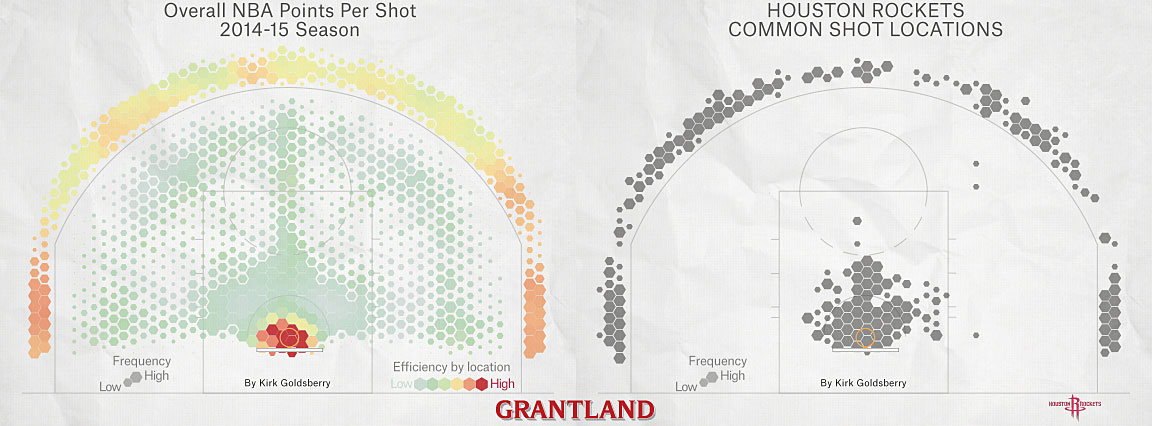
\includegraphics[width=18cm]{houston_shots.jpg}
	\caption{Decyzje rzutowe Houston i reszty ligi}\label{houston_shots}
	\centering
\end{figure}
 Poza analizowaniem przebiegu gry, analitycy oraz statystycy podejmują próby przewidywania wyników sezonu, co staje się bardzo istotne w razie kontuzji lub wymiany gracza\cite{replayNBA} \cite{graphicalNBA}. Niemal wszystkie zaproponowane dotąd modele symulacji rozgrywek opierają się na statystykach zawodników, ich wpływie na atak i obronę, udziale w zwycięstwach, oraz ulubionych pozycjach rzutowych. \\
 
 Celem pracy inżynierskiej jest próba przewidzenia rezultatów wybranego sezonu ligi NBA przy pomocy prostego modelu, używając wyłącznie informacji o wynikach poszczególnych drużyn z poprzednich sezonów --- indywidualny wpływ graczy na przebieg spotkań nie jest rozpatrywany. Na potrzeby tego zadania zaprojektowano kilka algorytmów opierających się na metodzie bootstrap, sprawdzono ich skuteczność dla kilku wybranych sezonów w zależności od okresu używanych danych i nadanych wag, a następnie przy pomocy najskuteczniejszych modeli dokonano predykcji wyników trwającego sezonu 2018/2019. 



\chapter{Opis ligi NBA}\label{rodzial1}
NBA (National Basketball Association) została założona 6 czerwca 1946 roku. Pierwotnie była znana jako Basketball Association of America i składała się z 11 zespołów, a swoją obecną nazwę zyskała w roku 1949, kiedy to wchłonęła konkurencyjną National Basketball League. Kolejna fuzja z inną ligą miała miejsce w 1976 roku, a mianowicie połączenie z bardziej widowiskową American Basketball Association. Po tym wydarzeniu NBA znacznie zyskała na atrakcyjności --- z ABA zaczerpnięto pomysł rzutów za trzy punkty oraz organizację konkursu wsadów, jak i przyjęto cztery dodatkowe kluby\cite{history}. Od 2004 roku w lidze gra 30 zespołów, 29 ze Stanów Zjednoczonych i 1 z Kanady. Liga podzielona jest na dwie konferencje po 15 drużyn, te natomiast składają się z dywizji po 5 organizacji. Szczegółowy podział na konferencje i dywizje, oraz nazwy wszystkich drużyn zawarte zostały w tabelach \ref{tabela_wschod} i \ref{tabela_zachod}, natomiast dokładne rozmieszczenie na mapie kontynentu znajduje się na rysunku \ref{mapa_stany}\cite{mapa}.

\begin{figure}[t]
	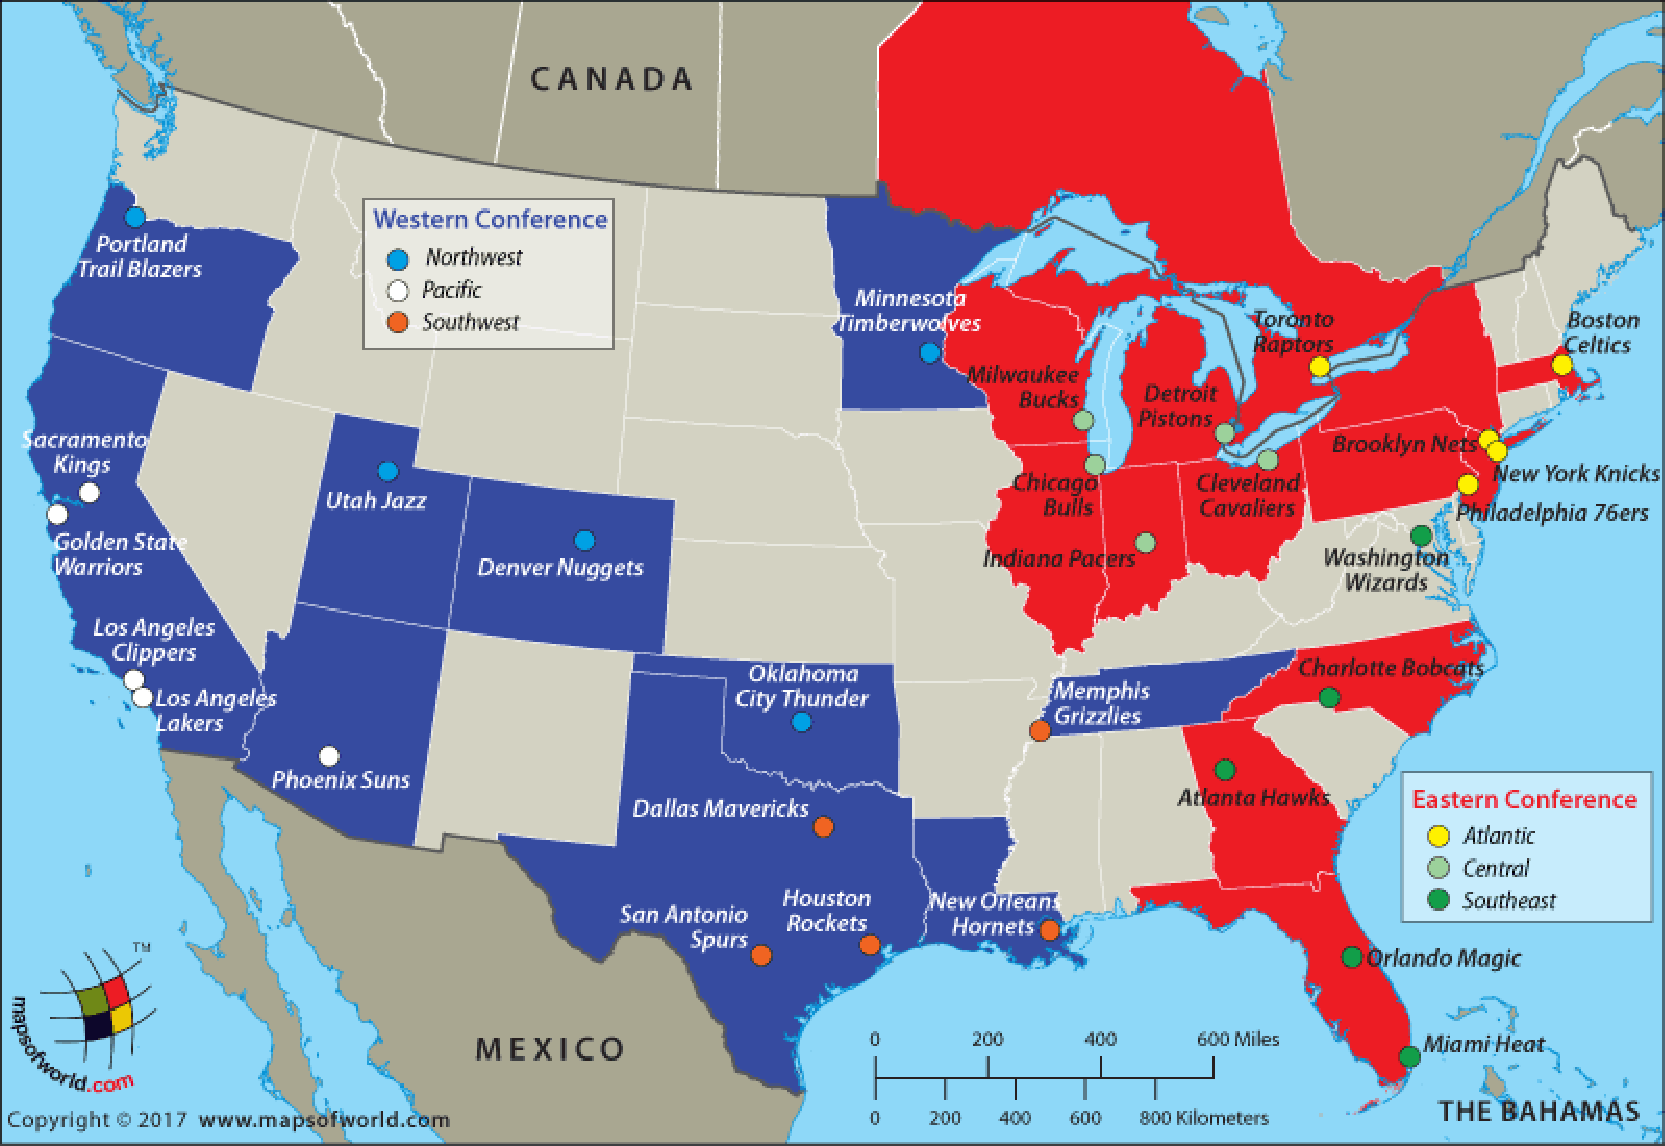
\includegraphics[width=16cm]{conf_map.pdf}
	\caption{Rozmieszczenie drużyn NBA}\label{mapa_stany}
	\centering
\end{figure}

\begin{table}[]
\begin{tabular}{ |p{5cm}|p{5cm}|p{5cm}|  }
	\hline
	\multicolumn{3}{|c|}{\textbf{Konferencja Wschodnia}} \\
	\hline
	\textbf{Atlantic Division}& \textbf{Southeast Division}&\textbf{Central Division}\\
	\hline
	Boston Celtics (BOS)& Atlanta Hawks (ATL)&Chicago Bulls (CHI)\\\hline
	Brooklyn Nets (BRK)&Charlotte Hornets (CHO)&Cleveland Cavaliers (CLE)\\\hline
	New York Knicks (NYK)&Miami Heat (MIA)&Detroit Pistons (DET)\\\hline
	Philadelphia 76ers (PHI)&Orlando Magic (ORL)&Indiana Pacers (IND)\\\hline
	Toronto Raptors (TOR)&Washington Wizards (WAS)&Milwaukee Bucks (MIL)\\\hline
\end{tabular}
\caption{Drużyny Konferencji Wschodniej}\label{tabela_wschod}
\end{table}
\begin{table}[]
\begin{tabular}{ |p{5.8cm}|p{5.4cm}|p{5.6cm}|  }
	\hline
	\multicolumn{3}{|c|}{\textbf{Konferencja Zachodnia}} \\
	\hline
	\textbf{Northwest Division}& \textbf{Southwest Division}&\textbf{Pacific Division}\\
	\hline
	Denver Nuggets (DEN)& Dallas Mavericks (DAL)&Golden State Warriors (GSW)\\\hline
	Minnesota Timberwolves (MIN)&Houston Rockets (HOU)&Los Angeles Clippers (LAC)\\\hline
	Oklahoma City Thunder (OKC)&Memphis Grizzlies (MEM)&Los Angeles Lakers (LAL)\\\hline
	Portland Trail Blazers (POR)&New Orleans Pelicans (NOP)&Phoenix Suns (PHX)\\\hline
	Utah Jazz (UTA)&San Antonio Spurs (SAS)&Sacramento Kings (SAC)\\
	\hline
\end{tabular}
\caption{Drużyny Konferencji Zachodniej}\label{tabela_zachod}
\end{table}
Dodatkowo, od 2004 roku niektóre kluby zmieniły swoje nazwy lub lokalizacje. W niektórych historycznych zestawieniach lub zbiorach danych mogą widnieć jako (podane w formacie nazwa obecna --- poprzednia):
\begin{itemize}
	\item Charlotte Hornets --- Charlotte Bobcats
	\item Brooklyn Nets --- New Jersey Nets
	\item Oklahoma City Thunder --- Seattle SuperSonics
	\item New Orleans Pelicans --- New Orleans Hornets
\end{itemize}

Sezon w NBA składa się z dwóch części: zasadniczej i następującej po niej pucharowej (playoffs). W sezonie zasadniczym każda drużyna rozgrywa 82 mecze, grając z każdym innym zespołem od 2 do 4 gier. Przykładowa tabela z wynikami na zakończenie sezonu została zawarta w tabeli \ref{tabela_wygrane_rzeczywiste}. Terminarz rozgrywek wyznaczany jest wedle następujących reguł:
\begin{enumerate}
	\item drużyny z różnych konferencji grają ze sobą 2 spotkania (1 na wyjeździe i 1 na własnym boisku),
	\item drużyny z tej samej dywizji grają ze sobą 4 spotkania (2 na wyjeździe i 2 na własnym boisku),
	\item drużyny z tej samej konferencji oraz różnych dywizji grają ze sobą 3 albo 4 spotkania (przynajmniej po jednym na wyjeździe i własnym boisku).
\end{enumerate}
Mecze koszykówki nie mogą zakończyć się remisem (w razie remisu po regulaminowym czasie gry rozgrywa się dogrywki aż do wyłonienia zwycięzcy).
Po zakończeniu sezonu następuje wspomniana wyżej faza pucharowa; wchodzi do niej po 8 najlepszych zespołów z każdej konferencji (w razie takiej samej ilości zwycięstw dla obu zespołów decydują wyniki ich bezpośrednich spotkań). W tej fazie drużyny grają ze sobą maksymalnie 7 meczów, czyli zespół, który pierwszy wygra 4 mecze, przechodzi do następnego etapu. W fazie playoff jasno zdefiniowane są lokalizacje odgrywania spotkań --- lepszy bilans zwycięstw w sezonie zasadniczym skutkuje przewagą parkietu. Seria spotkań grana jest w formacie 2–2–1–1–1, czyli mecze numer 1, 2, 5 i 7 grane są u lepszej z drużyn. Przy doborze przeciwników bierze się pod uwagę pozycję w tabeli konferencji: drużyna z miejsca pierwszego gra z zespołem na ósmym miejscu, druga z siódmą, i tak dalej. Zwycięzca serii przechodzi do następnego etapu z czterema drużynami, po którym następują finały konferencji --- najlepsze drużyny ze swoich grup spotykają się w finałach NBA. Dla lepszego zrozumienia systemu rozgrywek pucharowych na rysunku \ref{po_tree} zamieszczono tzw. ,,drzewko playoff''\cite{playoffs}, czyli grafikę oddającą przebieg tej fazy.
\begin{figure}[t]
	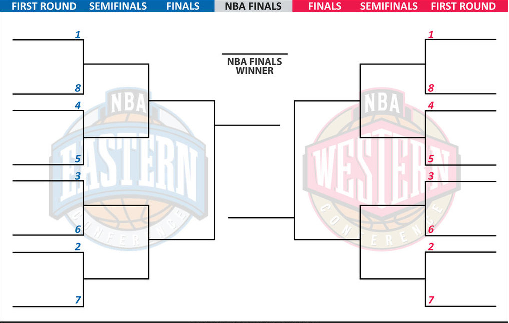
\includegraphics[width=16cm]{po_tree.pdf}
	\caption{Grafika obrazująca system rozgrywek pucharowych}\label{po_tree}
	\centering
\end{figure}
\begin{table}[]
	\centering
\begin{tabular}{|c|c|c|}
	\hline
	\textbf{Drużyna}      & \textbf{Zwycięstwa w sezonie 14/15} & \textbf{Zwycięstwa w sezonie 17/18} \\ \hline
	Atlanta Hawks & 60 & 24\\ \hline
	Boston Celtics & 40 & 55\\ \hline
	Brooklyn Nets & 38 & 28\\ \hline
	Charlotte Hornets & 33 & 36\\ \hline
	Chicago Bulls & 50 & 27\\ \hline	
	Cleveland Cavaliers & 53 & 50\\ \hline
	Dallas Mavericks & 50 & 24\\ \hline	
	Denver Nuggets & 30& 46\\ \hline
	Detroit Pistons & 32 & 39\\ \hline
	Golden State Warriors & 67 & 58\\ \hline
	Houston Rockets & 56 & 65 \\\hline
	Indiana Pacers & 38 & 48 \\\hline
	Los Angeles Clippers & 56 & 42\\ \hline
	Los Angeles Lakers & 21 & 35\\ \hline
	Memphis Grizzlies & 55 & 22\\ \hline
	Miami Heat & 37 & 44 \\\hline
	Milwaukee Bucks & 41 & 44\\ \hline
	Minnesota Timberwolves & 16 & 47\\ \hline
	New Orleans Pelicans & 45 & 48\\ \hline
	New York Knicks & 17 & 29\\ \hline
	Oklahoma City Thunder & 45 & 48\\ \hline
	Orlando Magic & 25 & 17\\ \hline
	Philadelphia 76ers & 18 & 52\\ \hline
	Phoenix Suns & 39 & 21 \\\hline
	Portland Trail Blazers & 51 & 49\\ \hline	
	Sacramento Kings & 29 & 27\\ \hline
	San Antonio Spurs & 55 & 47\\ \hline
	Toronto Raptors & 49 & 59\\ \hline
	Utah Jazz & 38 & 48 \\\hline
	Washington Wizards & 46 & 43\\ \hline
\end{tabular}
\caption{Liczby zwycięstw drużyn w wybranych sezonach}\label{tabela_wygrane_rzeczywiste}	
\end{table}
\\
\hspace*{6mm}Każdego lata, po zakończeniu fazy playoff, ma miejsce nabór młodych zawodników do NBA (tzw. Draft). Jest to okazja dla graczy uniwersyteckich, którzy chcieliby rozpocząć karierę zawodową, lub zawodników grających w innych ligach. Zasady Draftu są proste: każdy sportowiec może się do niego zgłosić tylko raz, oraz aby móc zagrać w lidze trzeba do niego obowiązkowo przystąpić --- jest to świetny sposób na utrzymanie balansu w NBA, ponieważ najlepsze zespoły mają najmniejsze szanse na otrzymanie praw do utalentowanych, młodych zawodników. Nabór nagradza najsłabsze kluby, ponieważ zespół z najgorszym wynikiem w sezonie zasadniczym ma największe szanse na otrzymanie pierwszego wyboru, druga najgorsza drużyna ma drugie największe szanse, i tak dalej. Kolejność wyborów jest ustalana poprzez losowanie, dlatego często w historii zdarzało się, że najsłabszy zespół nie uzyskał pierwszeństwa. Niestety, coraz częstszym zjawiskiem w NBA staje się tak zwane ,,tankowanie'', czyli celowe przegrywanie w celu uzyskania najwyższego możliwie wyboru w Drafcie. Zespoły na poziomie średniej ligowej, mając świadomość, że nie są w stanie walczyć o wysokie cele, decydują się na wejście w przebudowę i kilkuletnie poświęcanie zwycięstw na rzecz rozwoju młodzieży. Podczas porównywania wyników symulacji z rzeczywistymi w tej pracy, wielokrotnie można było zauważyć, które zespoły skupiły się na walce o młodych zawodników, a które o tytuły --- najlepszym wskaźnikiem tego jest liczba wygranych.

\chapter{Podstawowe pojęcia wykorzystane w pracy}

\section{Rozkład jednostajny}
\begin{definition}
Ciągła zmienna losowa $X$ ma rozkład jednostajny o parametrach $a$ i $b$, takich że $a,b\in \mathds{R}$ oraz $a<b$, oznaczany jako $\mathcal{U}(a,b)$ wtedy, gdy jej gęstość jest postaci
\begin{equation}
f(x)=\frac{1}{b-a}\mathds{1}_{(a,b)}(x) \cite{magiera}.
\end{equation}
\end{definition}
\noindent Wartość oczekiwana tego rozkładu wynosi
\begin{equation}
E(X)=\frac{a+b}{2},
\end{equation}
natomiast wariancja jest równa
\begin{equation}
Var(X)=\frac{(b-a)^2}{12}.
\end{equation} 
Funkcja charakterystyczna tego rozkładu wyrażona jest wzorem
\begin{equation}
\phi(t)=\frac{e^{itb}-e^{ita}}{(b-a)it}.
\end{equation}
W przypadku, gdy zmienna losowa $X$ posiada ciągłą dystrybuantę $F(x)$, to $U=F(x)$ ma rozkład $\mathcal{U}(0,1)$.

\section{Generatory liczb pseudolosowych rozkładu jednostajnego} %(str 427)
Załóżmy, że $F$ to dystrybuanta rozkładu jednostajnego $\mathcal{U}(0,1)$ \cite{koronacki}.  Podczas generowania ciągu zbliżonego do realizacji rozkładu jednostajnego zazwyczaj stosuje się następującą metodę: wybierzmy funkcję $G$ określoną i mającą wartości na odcinku $[0,1]$, o wartości początkowej $u_0 \in [0,1]$, i zdefiniujmy
\begin{equation}
	u_1=G(u_0), \,\, u_2=G(u_1), \,\, \dots, \,\,u_i=G(u_{i-1}), \,\, i=1,\,2,\,\dots 
\end{equation}
Znając postać funkcji $G$ i początkową wartość $u_0$ możliwe jest ponowne wygenerowanie każdego elementu zdefiniowanego powyżej ciągu. Prowadzi to do następującej definicji:
\begin{definition}
	Generator liczb pseudolosowych z rozkładu jednostajnego $\mathcal{U}(0,1)$ to taki algorytm dla funkcji $G$ o wartości startowej $u_0 \in [0,1]$, który wyznacza wartości $u_n$, mając przy okazji podaną własność: dla każdego $n$, wygenerowane $u_1,u_2,\dots,u_n$ oddają zachowanie próby losowej $U_1,U_2,\dots,U_n \sim \mathcal{U}(0,1)$ (popularne testy nie odrzucają hipotezy, wedle której $u_1,u_2,\dots,u_n$ to realizacja próby $U_1,U_2,\dots,U_n \sim \mathcal{U}(0,1)$).
\end{definition}

\section{Metoda Monte Carlo}
Załóżmy, że $\theta$ to parametr zmiennej losowej $X$ oraz można go przedstawić jako $\theta=Eh(X)$, przy czym $h$ to pewna znana funkcja, dodatkowym założeniem jest to, że można wygenerować próbę o rozkładzie $X$\cite{monte}.
\begin{definition}
	Niech $X_1,X_2,\dots,X_m$ będzie próbą pseudolosową pewnego rozkładu $X$ dla pewnego $m$. Średnia $\bar{h}=m^{-1}(h(X_1)+h(X_2)+\dots +h(X_m))$ nazywana jest \textbf{estymatorem $Eh(X)=\theta$ wyznaczonym metodą Monte Carlo}.
\end{definition}
Można zauważyć, że $\bar{h}$ to średnia próbkowa próby $h(X_1),h(X_2),\dots ,h(X_m)$, użycie jej do oszacowania parametru $\theta$ jest możliwe dzięki prawu wielkich liczb. Głównym problemem tego zagadnienia jest estymacja parametru $\theta$, który nie musi posiadać interpretacji probabilistycznej. Całość tej metody opiera się na generowaniu próby losowej lub pseudolosowej z rozkładu jednostajnego, zastosowaniu funkcji $h$ do przekształcenia elementów tej próby, a następnie wyznaczeniu estymatora $\bar{h}$ parametru $\theta$. 
W celu dokładnego opisania metody posłużmy się przykładem: obliczmy
\begin{equation}
	\theta:=\int_{0}^{1}g(x)\,dx.
\end{equation}
W przypadku, gdy nie jesteśmy w stanie policzyć tej całki analitycznie, pozostaje nam zastosowanie metod numerycznych lub symulacyjnych. Algorytm szacowania parametru $\theta$ przy użyciu metody Monte Carlo:
\begin{enumerate}
	\item wygeneruj $U_1,U_2,\dots, U_n \sim \text{IID}\,\,\,\, \mathcal{U}(0,1)$,
	\item oszacuj $\theta$ korzystając z
	\begin{equation}
		\hat{\theta}_n:= \frac{g(U_1)+g(U_2)+\dots+g(U_n)}{n}.
	\end{equation}
\end{enumerate} 

Modelowanie przy pomocy metody Monte Carlo jest przydatne przy badaniu skomplikowanych procesów losowych, które można rozbić na dwie kategorie. Pierwsza skupia w sobie systemy, w których proces jest sprecyzowany, ale poprzez jego złożoność trudno obliczyć jego parametry teoretyczne. Druga kategoria to eksperymenty losowe o modelu matematycznym trudnym do skonstruowania --- dzięki metodzie Monte Carlo można dokonać ich klasyfikacji generując wyniki modelowe, po czym przyrównać je z danymi eksperymentalnymi. Omawiana w następnym rozdziale metoda bootstrap w swoich założeniach wywodzi się z symulacji Monte Carlo.

\section{Zasada bootstrap}
%In statistics, bootstrapping is any test or metric that relies on random sampling with replacement.
Próba bootstrap to metoda służąca do oceny rozkładu pewnego estymatora (na przykład wariancji)  używając wielokrotnych symulacji opartych na znanej realizacji jego rozkładu. Narzędzie to zostało stworzone przez Bradleya Efrona i opublikowane w artykule ,,Bootstrap methods: another look at the jackknife'' z 1979 roku\cite{efron1}. Załóżmy, że $x_1, x_2 \dots x_n$ to realizacja pewnej próby losowej, a $\hat{F}$ jest dystrybuantą empiryczną tej próby. Dystrybuanta $\hat{F}$ to znane przybliżenie pewnego nieznanego rozkładu $F$, dlatego też rozkład $\hat{\Theta}$ estymować będziemy przy pomocy $\hat{F}$, czyli dokonamy oceny rozkładu estymatora $\hat{\Theta}$ w oparciu o generowanie prób z rozkładu $\hat{F}$\cite{koronacki}.
\begin{definition}
	Próba losowa $X^* = (X_1^*, X_2^*, \dots, X_n^*)$ o rozkładzie $\hat{F}$ dla ustalonej realizacji $x = (x_1, x_2, \dots, x_n)$ nazywana jest \textbf{próbą bootstrap}.
\end{definition}
Otrzymywanie realizacji próby bootstrap bazuje na wykonaniu $n$-krotnego losowania ze zwracaniem elementów próby pierwotnej, tak więc losowość w próbie $X^*$ polega na losowym wyborze elementu $x_1, x_2, \dots, x_n$. W ten sposób powstaje populacja, w której każda zmienna $X_i^*$ jest niezależna od pozostałych, oraz z jednakowym prawdopodobieństwem  przyjmuje dowolną wartość próby. Efron wykazał, że rozkład $T(X^*)$ dla ustalonych $x_1, x_2, \dots, x_n$ ma kształt zbliżony do rozkładu $T(X)$, ponadto rozkład statystyki $(T(X^*)-\hat{\Theta})$ jest bliski rozkładowi statystyki $(T(X)-\Theta)$. Dzięki temu można dokonać oceny rozkładu $\Theta=T(X)$ wykonując poniższe kroki:
\begin{enumerate}
	\item dokonaj losowania niezależnych prób bootsrap $X_1^*, X_2^*, \dots, X_k^*$ korzystając z realizacji $x_1, x_2, \dots, x_n$,
	\item wyznacz $\Theta_1^*=T(X_1^*)-\hat{\Theta}$, $\Theta_2^*=T(X_2^*)-\hat{\Theta}$, \dots, $\Theta_k^*=T(X_k^*)-\hat{\Theta}$.
\end{enumerate}
Otrzymany w ten sposób rozkład $(\Theta_1^*, \Theta_2^*, \dots, \Theta_k^*)$ to przybliżenie rozkładu błędów estymacji $\hat{\Theta}-\Theta$ przy pomocy statystyki $T$. Histogram tego rozkładu nazywany jest estymatorem rozkładu $\hat{\Theta}$ otrzymanym metodą bootstrap. Dla zadowalającego przybliżenia rozkładu $(T(X^*)-\hat{\Theta})$ wymagane jest przynajmniej $k=1000$ prób bootstrap, a im większa ich ilość, tym dokładniejsze oszacowanie.  

\subsection{Bootstrap parametryczny}
Założenia bootstrapu parametrycznego są podobne do bootstrapu klasycznego --- jedyną różnicą jest fakt, że zamiast symulowania niezależnych prób bootstrapowych z dystrybuanty empirycznej, generowane są niezależne próby z rozkładu pewnego parametrycznego modelu\cite{efron2}.
W tym przypadku do danych dopasowany jest pewien model teoretyczny (często przy pomocy metody największej wiarygodności), a próby liczb losowych generowane są z owego dopasowanego modelu. Proces symulowania tak zdefiniowanej próby przebiega podobnie do innych procesów bootstrapowych, przy czym wielkość takiej próby zazwyczaj odpowiada rozmiarowi oryginalnego zbioru danych. Prowadzi to do następującej definicji:
\begin{definition}
	Próbę bootstrap, której nieznany rozkład $F$ można przybliżyć pewnym znanym rozkładem parametrycznym $\hat{F}$ nazywamy \textbf{parametryczną próbą bootstrap}. 
\end{definition}
 
 
\chapter{Metodologia, algorytmy}\label{rodzial_algorytmy}
\section{Opis danych}
Dane, które będą wykorzystywane do symulacji sezonu, tak jak i terminarze, zostały zebrane ze strony sportowej \textit{basketballreference.com}\cite{dane}.
Na potrzeby tej pracy zebrano wyniki starć pomiędzy drużynami począwszy od sezonu 2004/2005 aż do 2017/2018. Początkowo symulowano rozgrywki sezonów 2014/2015 oraz 2017/2018 w celu wybrania najlepszego modelu, a następnie skorzystano z niego, aby przewidzieć wyniki rozgrywek we wciąż trwającym sezonie 2018/2019.
Posiadając ilość wygranych jednej drużyny z drugą na przestrzeni lat dokonano następujących transformacji danych:
\\
\hspace*{6mm}W zależności od przedziału czasowego, jaki będziemy rozpatrywać, zebrano wyniki w określonych rozgrywkach (na przykład, przy wyznaczaniu wyników sezonu 2014/2015 i przedziale 5 lat, używać będziemy danych z lat 2009 do 2014). Dzięki uzyskanej w ten sposób liczbie wygranych możemy wyznaczyć stosunek zwycięstw do porażek dla wybranych zespołów (przykład: Boston Celtics i Atlanta Hawks grały ze sobą 10 razy, druga z drużyn wygrała zaledwie 4 razy, dlatego też w starciu z Celtami ich szansa na wygraną wynosi $0.4$). Po zastosowaniu tej metody dla wszystkich zespołów uzyskano macierz o liczbie wierszy i kolumn odpowiadającej ilości drużyn w NBA, zawierającą prawdopodobieństwa na wygraną z każdym zespołem w lidze. Przykładowa postać danych zawarta została w tabeli \ref{dane_tabela}.
\begin{table}[]
	\centering
	\begin{tabular}{|c|c|c|c|}
		\hline
		&ATL & BOS & CHO\\ \hline
		ATL &  & 0.61&0.54\\ \hline
		BOS & 0.39 & &0.71\\ \hline
		CHO & 0.46 & 0.29&\\ \hline
	\end{tabular}
	\caption{Przykładowa tabela z danymi}\label{dane_tabela}	
\end{table}

Ze względu na formę użytych danych nie ma znaczenia, czy podczas symulacji wykorzystywany będzie bootstrap klasyczny lub parametryczny. Używanie pierwszego polegałoby na losowaniu ze zwracaniem wyników (zwycięstwo lub porażka) z danych historycznych --- jest to jednoznaczne z wyliczeniem prawdopodobieństwa wygranej w oparciu o historię i symulowaniu rozkładu dwupunktowego.

\section{Własne oznaczenia} \label{wlasne_oznaczenia}
Podczas prób symulacji dokonano intuicyjnego założenia, wedle którego największy wpływ na postawę sezonu mają rozgrywki bezpośrednio go poprzedzające. W tym celu dobrano system wag --- z powodu dynamicznych zmian w lidze, najstarsze sezony otrzymują najmniejszą rangę, która stopniowo zwiększa się, im bliżej do zawodów rozpatrywanych w symulacji. Ważona ilość zwycięstw $Z_{ij}$ $i-$tej drużyny $D_i$ z $j-$tą drużyną $D_j$ wynosi
\begin{equation}
	Z_{ij} = \sum_{k=1}^{n} (1+x\cdot k)\cdot R_{ijk}, 
\end{equation}
gdzie $n$ to ilość sezonów, z których pobrano dane, $x$ to ustalona waga kolejnych rozgrywek, a $R_{ijk}$ to wynik starć drużyny $D_i$ z drużyną $D_j$ w $k-$tym sezonie. Podczas testowania skuteczności modeli dobierano różne wagi w celu znalezienia tego zwracającego najlepsze predykcje. W trakcie symulacji program przechodzi przez dokładnie określony terminarz rozgrywek --- drużyna gra z przeciwnikiem tyle razy, ile spotkań wyznaczono w rozkładzie. Algorytmy losowania opisano szczegółowo w rozdziale \ref{rodzial1}. 
Na potrzeby testów mających na celu wyłonienie najlepszego modelu zdefiniowano współczynnik $G$ równy
\begin{equation}\label{wskaznik_g}
	G = \sum_{i=1}^{n}|\hat{\Theta_i} - \Theta_i|,
\end{equation}
gdzie $n$ to ilość drużyn (obecnie 30), $\hat{\Theta_i}$ to wartość estymowana przy pomocy próby bootstrap dla $i$-tej drużyny, a $\Theta_i$ to jej rzeczywisty wynik w porównywanym sezonie. Wartość $G$ to bezwzględna suma błędów modelu, a więc im jest ona mniejsza, tym lepsze jest dopasowanie. 

\section{Modele symulacji rozgrywek}
Zaproponowane w tym rozdziale modele opierają się na zasadzie bootstrapu parametrycznego. Przed rozpoczęciem symulacji znane są prawdopodobieństwa poszczególnych drużyn na wygraną, co pozwala na przybliżenie rozkładu teoretycznego danego sezonu. 

\subsection{Model I --- uśredniony}
Pierwszy ze stworzonych modeli polega na obliczeniu ogólnego stosunku zwycięstw do porażek dla każdej drużyny w wybranym okresie --- wszystkie wygrane zespołu zostają podzielone przez łączną liczbę rozegranych spotkań, wynikiem czego jest liczba z przedziału $[0,1]$ określana jako $P_{i}$, gdzie $i$ to $i-$ta drużyna. Schemat symulowania wyników spotkań między drużynami został szczegółowo opisany w algorytmie \ref{algorytm1} i pseudokodzie \ref{pseudokod1}.

\begin{algorytm} \label{algorytm1}
	\textbf{Model uśredniony}
	\begin{enumerate}
	\item wstaw liczniki zwycięstw drużyn $B_1= 0,B_2= 0,\dots, B_{30}= 0$
	\item dla $i=1$, $i=2$, \dots, $i=30$: 
	\begin{enumerate}
		\item dla $j=i$, $j=i+1$, \dots, $j=30$: 
		\begin{enumerate}
			\item znajdź drużyny $D_i$ i $D_j$
		\item odczytaj średnie ilości zwycięstw $W_i$ i $W_j$ dla drużyn $D_i$ i $D_j$ 
		\item wyznacz prawdopodobieństwo zwycięstwa $W_{ij}$ przez drużynę  $D_i$ równe $W_{ij}=\frac{W_i}{W_i + W_j}$   
		\item w terminarzu znajdź liczbę spotkań $S_{ij}$ pomiędzy drużynami $D_i$ i $D_j$
		\item wykonaj $S_{ij}$ razy:
			\begin{enumerate}
				\item symuluj liczbę $U$ z rozkładu jednostajnego $\mathcal{U}\sim U[0,1]$ 
			\item jeżeli $W_{ij} \leq U,$ to zwiększ licznik zwycięstw $B_i=B_i+1$, w przeciwnym razie zwiększ licznik zwycięstw $B_j=B_j+1$
			\end{enumerate}
		\end{enumerate}
	\end{enumerate}
\end{enumerate}
\end{algorytm} 
 
\begin{pseudokod} \label{pseudokod1}
	\textbf{Model uśredniony}
	\begin{algorithmic}[1]
		\State $B_1\gets 0,B_2\gets 0,\dots, B_{30}\gets 0$
		\State $i\gets 1$
		\While{$i\leq 30$}
		\For{$j\gets i$ to 30}
		\State znajdź drużyny $D_i$ i $D_j$
		\State znajdź $W_i$ i $W_j$ 
		\State $W_{ij}\gets\frac{W_i}{W_i + W_j}$
		\State znajdź liczbę spotkań $S_{ij}$ pomiędzy $D_i$ i $D_j$
		\For{$p\gets1$ to $S_{ij}$}
		\State $U\sim \mathcal{U}[0,1]$
		\If {$W_{ij} \leq U$}
		\State $B_i \gets B_i+1$
		\Else
		\State $B_j \gets B_j+1$
		\EndIf
		\EndFor
		\EndFor
		\State $i\gets i+1$
		\EndWhile
	\end{algorithmic}
\end{pseudokod}

\subsection{Model II --- rywalizacji}
Drugi z zaproponowanych modeli zakłada zwracanie uwagi na historyczne wyniki przeciwko konkretnej drużynie. W zawodowym sporcie niejednokrotnie można trafić na zażarte rywalizacje między dwoma klubami lub tendencję do wygrywania z pewnym przeciwnikiem. Schemat symulowania wyników przy wykorzystaniu tego modelu został szczegółowo opisany w algorytmie \ref{algorytm2} i pseudokodzie \ref{pseudokod2}.

\begin{algorytm} \label{algorytm2}
	\textbf{Model rywalizacji}
	\begin{enumerate}
		\item wstaw liczniki zwycięstw drużyn $B_1= 0,B_2= 0,\dots, B_{30}= 0$
		\item dla $i=1$, $i=2$, \dots, $i=30$: 
		\begin{enumerate}
			\item dla $j=i$, $j=i+1$, \dots, $j=30$: 
			\begin{enumerate}
				\item znajdź drużyny $D_i$ i $D_j$
				\item odczytaj z macierzy wyników stosunek zwycięstw $W_{ij}=\frac{Z_{ij}}{Z_{ij}+Z_{ji}}$ drużyny $D_i$ przeciwko drużynie $D_j$   
				\item w terminarzu znajdź liczbę spotkań $S_{ij}$ pomiędzy drużynami $D_i$ i $D_j$
				\item wykonaj $S_{ij}$ razy:
				\begin{enumerate}
					\item symuluj liczbę $U$ z rozkładu jednostajnego $\mathcal{U}\sim U[0,1]$ 
					\item jeżeli $W_{ij} \leq U,$ to zwiększ licznik zwycięstw $B_i=B_i+1$, w przeciwnym razie zwiększ licznik zwycięstw $B_j=B_j+1$
				\end{enumerate}
			\end{enumerate}
		\end{enumerate}
	\end{enumerate}
\end{algorytm} 

\begin{pseudokod} \label{pseudokod2}
	\textbf{Model rywalizacji}
	\begin{algorithmic}[1]
		\State $B_i\gets 0,B_j\gets 0,\dots, B_{30}\gets 0$
		\State $i\gets 1$
		\While{$i\leq 30$}
		\For{$j\gets i$ to 30}
		\State znajdź drużyny $D_i$ i $D_j$
		\State znajdź $Z_{ij}$ i $Z_{ji}$ 
		\State $W_{ij}=\frac{Z_{ij}}{Z_{ij}+Z_{ji}}$
		\State znajdź liczbę spotkań $S_{ij}$ pomiędzy $D_i$ i $D_j$
		\For{$p\gets1$ to $S_{ij}$}
		\State $U\sim \mathcal{U}[0,1]$
		\If {$W_{ij} \leq U$}
		\State $B_i \gets B_i+1$
		\Else
		\State $B_j \gets B_j+1$
		\EndIf
		\EndFor
		\EndFor
		\State $i\gets i+1$
		\EndWhile
	\end{algorithmic}
\end{pseudokod}

\subsection{Model III --- fazy pucharowej}
Po symulacji całego sezonu, czyli 1230 spotkań, 8 najlepszych drużyn z każdej konferencji przechodzi do fazy playoff, gdzie toczy rozgrywki zgodnie z systemem opisanym w rozdziale \ref{rodzial1}. Na tym etapie rozgrywek symulacja spotkań różni się od części zasadniczej: zamiast jednego z zasugerowanych powyżej modeli korzysta się ze wcześniejszej symulacji fazy zasadniczej. W celu oddania trendów panujących w wygenerowanych rozgrywkach (potencjalnych kontuzjach, spadkach lub zwyżkach formy), użyta zostaje jedynie informacja o ilości wygranych przed rozpoczęciem playoffów. Szczegółowy opis symulacji tej fazy został opisany w algorytmie \ref{algorytm3} i pseudokodzie \ref{pseudokod3}.

\begin{algorytm} \label{algorytm3}
	\textbf{Model playoff}
	\begin{enumerate}
		\item wybierz drużyny $D_i$ i $D_j$
		\item wstaw liczniki zwycięstw $ZW_i=0$ i $ZW_j=0$
		\item odczytaj symulowane ilości zwycięstw z sezonu zasadniczego $B_i$ i $B_j$ dla wybranych drużyn $D_i$ i $D_j$
		\item wyznacz prawdopodobieństwo zwycięstwa drużyny $D_i$ nad drużyną $D_j$ równe $W_{ij}=\frac{B_i}{B_i + B_j}$
		\item powtarzaj dopóki  $ZW_i=4$ albo $ZW_j=4$:
		\begin{enumerate}
			\item symuluj liczbę $U$ z rozkładu jednostajnego $U\sim U[0,1]$ 
			\item jeżeli $W_{ij} \leq U,$ wstaw $ZW_i=ZW_i+1$, w przeciwnym razie wstaw $ZW_j=ZW_j+1$
		\end{enumerate}
		\item jeżeli $ZW_i=4$, to przenieś drużynę $D_i$ do następnego etapu, w przeciwnym razie przenieś drużynę $D_j$
	\end{enumerate}
\end{algorytm} 

\begin{pseudokod} \label{pseudokod3} 
	\textbf{Model playoff}
	\begin{algorithmic}[1]
		\State znajdź drużyny $D_i$ i $D_j$
		\State $ZW_i\gets 0,ZW_j\gets 0$
		\State znajdź $B_{i}$ i $B_{j}$ 
		\State $W_{ij}=\frac{B_i}{B_i + B_j}$
		\While{$ZW_i<4$ and $ZW_j<4$}
		\State $U\sim \mathcal{U}[0,1]$
		\If {$W_{ij} \leq U$}
		\State $B_i \gets B_i+1$
		\Else
		\State $B_j \gets B_j+1$
		\EndIf
		\EndWhile
		\If {$ZW_i=4$}
		\State $D_i$ przechodzi do następnej rundy
		\Else
		\State $D_j$ przechodzi do następnej rundy
		\EndIf
	\end{algorithmic}
\end{pseudokod}

Ilości zwycięstw drużyn w kolejnych symulowanych rozgrywkach są zapisywane i zapamiętywane, podobnie jak informacje o przejściach do kolejnych faz rozgrywek pucharowych. 

\section{Predykcja wyników na podstawie symulacji}
Korzystając z metod bootstrapowych zaproponowano kilka modeli pozwalających na oszacowanie przebiegu rozgrywek w analizowanym sezonie.
Przed korzystaniem z opisanych poniżej schematów przeprowadzono symulację opartą na algorytmach zdefiniowanych w rozdziale \ref{rodzial_algorytmy}, dzięki czemu do symulacji podchodzono z przygotowanymi wcześniej danymi.

\subsection{Predykcja wyników sezonu zasadniczego} \label{predykcja_zasadniczego}
Sezon zasadniczy odgrywa bardzo ważną rolę w rozgrywkach NBA --- w trakcie jego trwania drużyny toczą walkę o najlepsze miejsca w fazie pucharowej, sprawdzają swoje siły w trakcie gier z potencjalnymi rywalami w playoff, a także wzmacniają swoje drużyny poprzez rotację zawodników. Podczas przejść symulacji zapisywano łączną liczbę wygranych każdego zespołu, dzięki czemu otrzymano rozkłady zwycięstw wszystkich składów. Po przeanalizowaniu rozkładów zauważono, że mediany i wartości średnie nie różnią się znacznie od siebie, dlatego w dalszych rozważaniach jako przyszłą liczbę wygranych zespołu w sezonie zasadniczym przyjmuje się medianę rozkładu zwycięstw w symulacji. Wyniki porównania zawarto w tabeli \ref{srednie_mediany}. Dodatkowo zbadano normalność rozkładów zwycięstw wszystkich drużyn. Niestety, pomimo kształtu gęstości zbliżonego do normalnego, wszystkie testy statystyczne odrzuciły hipotezę o rozkładzie normalnym.
\begin{table}[]
	\centering
	\begin{tabular}{|c|c|c|}
		\hline
		\textbf{Drużyna}      & \textbf{Mediana} & \textbf{Średnia} \\ \hline
		ATL & 47 & 46.95\\ \hline
		BOS & 44 & 44.13\\ \hline
		CHO & 39 & 39.07\\ \hline
		CHI & 44 & 43.97\\ \hline
		CLE & 49 & 49.13\\ \hline
		DAL & 41 & 41.53\\ \hline
		DEN & 36 & 36.18\\ \hline
		DET & 36 & 35.97\\ \hline
		GSW & 65 & 65.09\\ \hline
		HOU & 51 & 50.96\\ \hline
		IND & 43 & 43.57\\ \hline
		LAC & 54 & 53.97\\ \hline
		LAL & 24 & 23.98\\ \hline
		MEM & 47 & 47.20\\ \hline
		MIA & 46 & 45.59\\ \hline
		MIL & 36 & 28.79\\ \hline
		MIN & 29 & 35.97\\ \hline
		BRK & 29 & 29.23\\ \hline
		NOP & 35 & 34.73\\ \hline
		NYK & 31 & 30.99\\ \hline
		ORL & 28 & 28.33\\ \hline
		PHI & 21 & 20.83\\ \hline
		POR & 45 & 45.09\\ \hline
		SAC & 31 & 31.06\\ \hline
		SAS & 61 & 61.38\\ \hline
		OKC & 51 & 51.16\\ \hline
		TOR & 50 & 50.36\\ \hline
		UTA & 41 & 41.46\\ \hline
		WAS & 44 & 43.80\\ \hline
	\end{tabular}
\caption{Porównanie średnich i median wygranych spotkań w symulacji}\label{srednie_mediany}	
\end{table}
\subsection{Modele predykcji wyników fazy pucharowej}\label{modele_palyoff}
Rozgrywki playoff są niezwykle trudne do przewidzenia --- niejednokrotnie zdarzyło się, że faworyci zostali pokonani przez znacznie niżej notowanego przeciwnika (najlepszy przykład to seria DAL-GSW w 2007 roku, kiedy Dallas Mavericks kończąc sezon z najlepszym bilansem zwycięstw w lidze, przegrali pierwszą rundę w 6 meczach z ósmą drużną konferencji).
Do symulacji tego etapu zaproponowano 2 odmienne od siebie modele, bazujące na innych założeniach.

\subsubsection{Model IV --- Prawdopodobieństwo przejść}
Model ten polega na oszacowaniu szans poszczególnych drużyn na przejście do wybranych etapów rozgrywek pucharowych. Podczas każdej z symulacji sezonu zbierano informacje o przejściach zespołów do kolejnych faz playoff. W ten sposób estymowano prawdopodobieństwa przejść do odpowiednio pierwszej rundy, drugiej rundy, finałów konferencji oraz finałów. Według zaproponowanego schematu do kolejnych etapów awansują zespoły z największą ilością przejść, a więc największym prawdopodobieństwem awansu. Do rundy pierwszej każdej konferencji dostanie się 8 drużyn najczęściej zakwalifikowanych w symulacjach, do drugiej 4 zespoły o największym prawdopodobieństwie przejścia do drugiego etapu, kolejne etapy wyznaczane są analogicznie. 

\subsubsection{Model V --- Najczęstsze kombinacje}
Drugi z badanych modeli porównuje najczęściej pojawiające się kombinacje zespołów w poszczególnych etapach. Podczas symulacji rozgrywek pucharowych zapisywano listy z drużynami przechodzącymi do kolejnych etapów playoff, dzięki czemu zachowane zostały również układy, w jakich toczyły się rozgrywki. Innymi słowy, dla rundy pierwszej wyszukiwana jest najczęściej pojawiająca się kombinacja zespołów w pierwszej rundzie, czynność ta jest powtarzana w kolejnych etapach. Mechanizm ten jest w stanie zwrócić bardzo precyzyjną prognozę, wymaga jednak dużej liczby powtórzeń symulacji do poprawnego działania. 

\chapter{Symulacje}
\section{Dobór optymalnego modelu}
Podczas testowania modeli badano zmiany wag poszczególnych sezonów oraz okres zbierania danych. Podjęto decyzję o przeprowadzaniu symulacji dla sezonów 2014/2015 oraz 2017/2018 o następujących parametrach:
\begin{itemize}
	\item wagi wynoszące odpowiednio $x=0$, $x=0.5$, $x=1$,
	\item okresy zbierania danych wynoszące odpowiednio 5 i 10 lat, a zatem
	\begin{itemize}
		\item dla sezonu 2014/2015 wykorzystywano dane z lat 2009-2014 oraz 2004-2014
		\item dla sezonu 2017/2018 wykorzystywano dane z lat 2012-2017 oraz 2007-2017
	\end{itemize}
\end{itemize}
Wszystkie przeprowadzone w ten sposób symulacje zostały wykonane dla 10000 powtórzeń próby bootstrap. 

\subsection{Wyniki symulacji dla sezonów zasadniczych}
Podczas symulowania podstawowej części sezonu, jako przewidzianą liczbę wygranych przyjęto medianę rozkładu symulowanych zwycięstw, co zostało opisane w Podrozdziale \ref{predykcja_zasadniczego}. Przy pomocy czynnika $G$ zdefiniowanego w rozdziale \ref{wskaznik_g} dokonano oceny modeli dla określonych wcześniej parametrów. Dodatkowo obliczono sumę błędów dla obu badanych sezonów, co znacznie uprości wybór lepszego modelu. Wyniki symulacji zawarto w tabeli \ref{tabela_porownianie_modeli}.
\begin{table}[]
	\centering
	\begin{tabular}{|c|c|c|c|}
		\hline
		\textbf{Parametry} & \textbf{Sezon 14/15} & \textbf{Sezon 17/18} & \textbf{Suma} \\ \hline
		M I, 5 lat, waga $0$ & 306  & 280 & 586\\ \hline
		M I, 5 lat, waga $0,5$ & 295 & 275 & 570 \\ \hline
		M I, 5 lat, waga $1$ & 293 & 270 & 563\\ \hline
		M I, 10 lat, waga $0$ & 318 & 290 & 608\\ \hline
		M I, 10 lat, waga $0,5$ & 304 & 275 & 579\\ \hline
		M I, 10 lat, waga $1$ & 303 & 283 & 586\\ \hline
		M II, 5 lat, waga $0$ &  304 & 308 & 612\\ \hline
		M II, 5 lat, waga $0,5$ & 305 & 292 & 597\\ \hline
		M II, 5 lat, waga $0$ & 305 & 289 & 594\\ \hline
		M II, 10 lat, waga $0$ & 331 & 299 & 630\\ \hline
		M II, 10 lat, waga $0,5$& 314 & 275 & 589 \\ \hline
		M II, 10 lat, waga $1$ & 331 & 298 & 629 \\ \hline
	\end{tabular}
	\caption{Współczynnik $G$ jakości dopasowania modelu}\label{tabela_porownianie_modeli}	
\end{table}
Jak można zauważyć, najlepsze oceny otrzymał Model I dla danych z 5 lat i wagą $x=1$. Do dalszych rozważań zakwalifikowany został również Model 2 z zebranymi 10 sezonami o wadze $x=0.5$ (okazał być się najlepszy w prognozie drugiego symulowanego sezonu). Pomimo gorszej oceny, korzystne będzie przetestowanie dwóch różnych modeli w następnym etapie. Po przeanalizowaniu rezultatów symulacji okazało się, że wyniki dla sezonu 2017/2018 były znacznie lepsze niż dla 2014/2015. Na rysunkach \ref{m1_5lat_waga1_wschod_17}--\ref{m2_10lat_waga05_zachod_17} zawarto wykresy pudełkowe wygenerowanych rozkładów zwycięstw dla wszystkich drużyn w sezonie 2017/2018 przy użyciu wybranych wcześniej modeli i parametrów. 

\begin{figure}[t]
	\hspace*{-3cm}  
	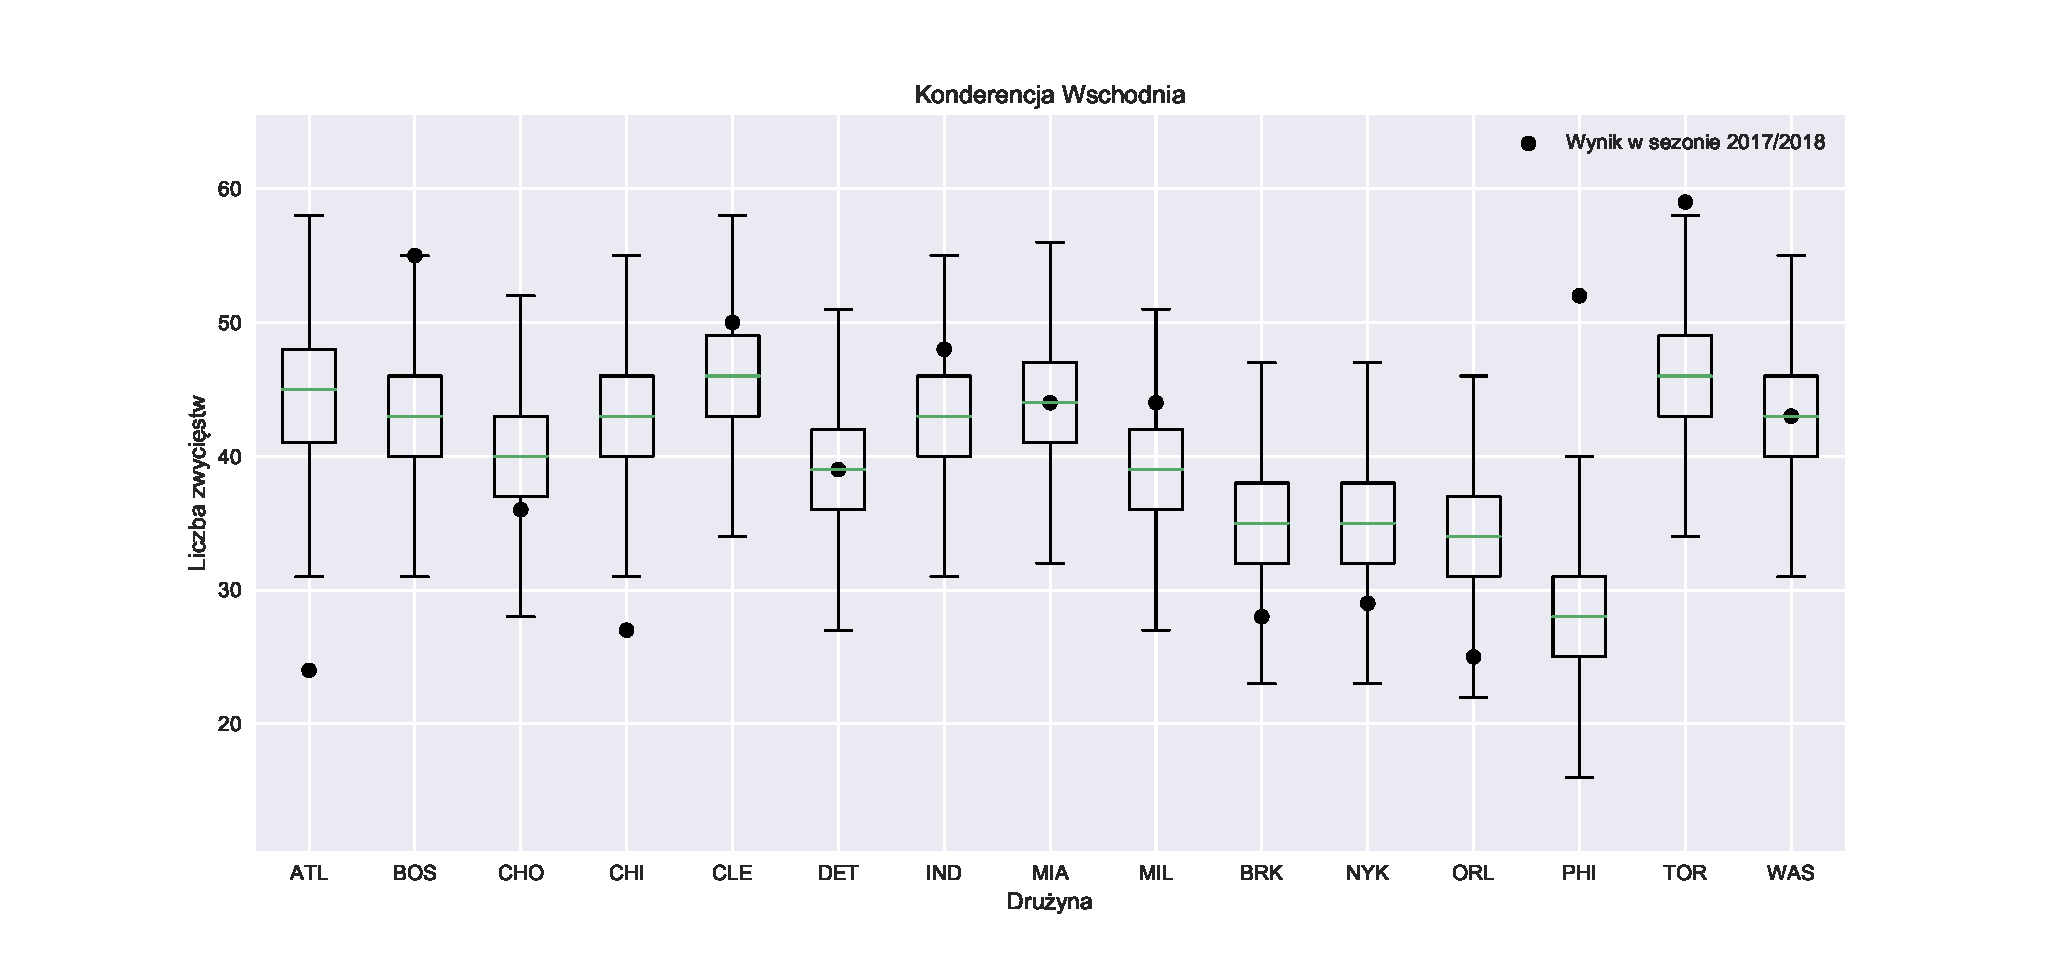
\includegraphics[width=22cm]{m1_dla17_5lat_waga1_box_wschod.pdf}
	\caption{Wykres pudełkowy wyników symulacji sezonu przy użyciu modelu I, na podstawie danych z 5 lat i wadze $x=1$, Konferencja Wschodnia}%Model I, 5 lat, waga 1
	\label{m1_5lat_waga1_wschod_17}
	\centering
\end{figure}

\begin{figure}[t]
	\hspace*{-3cm}  
	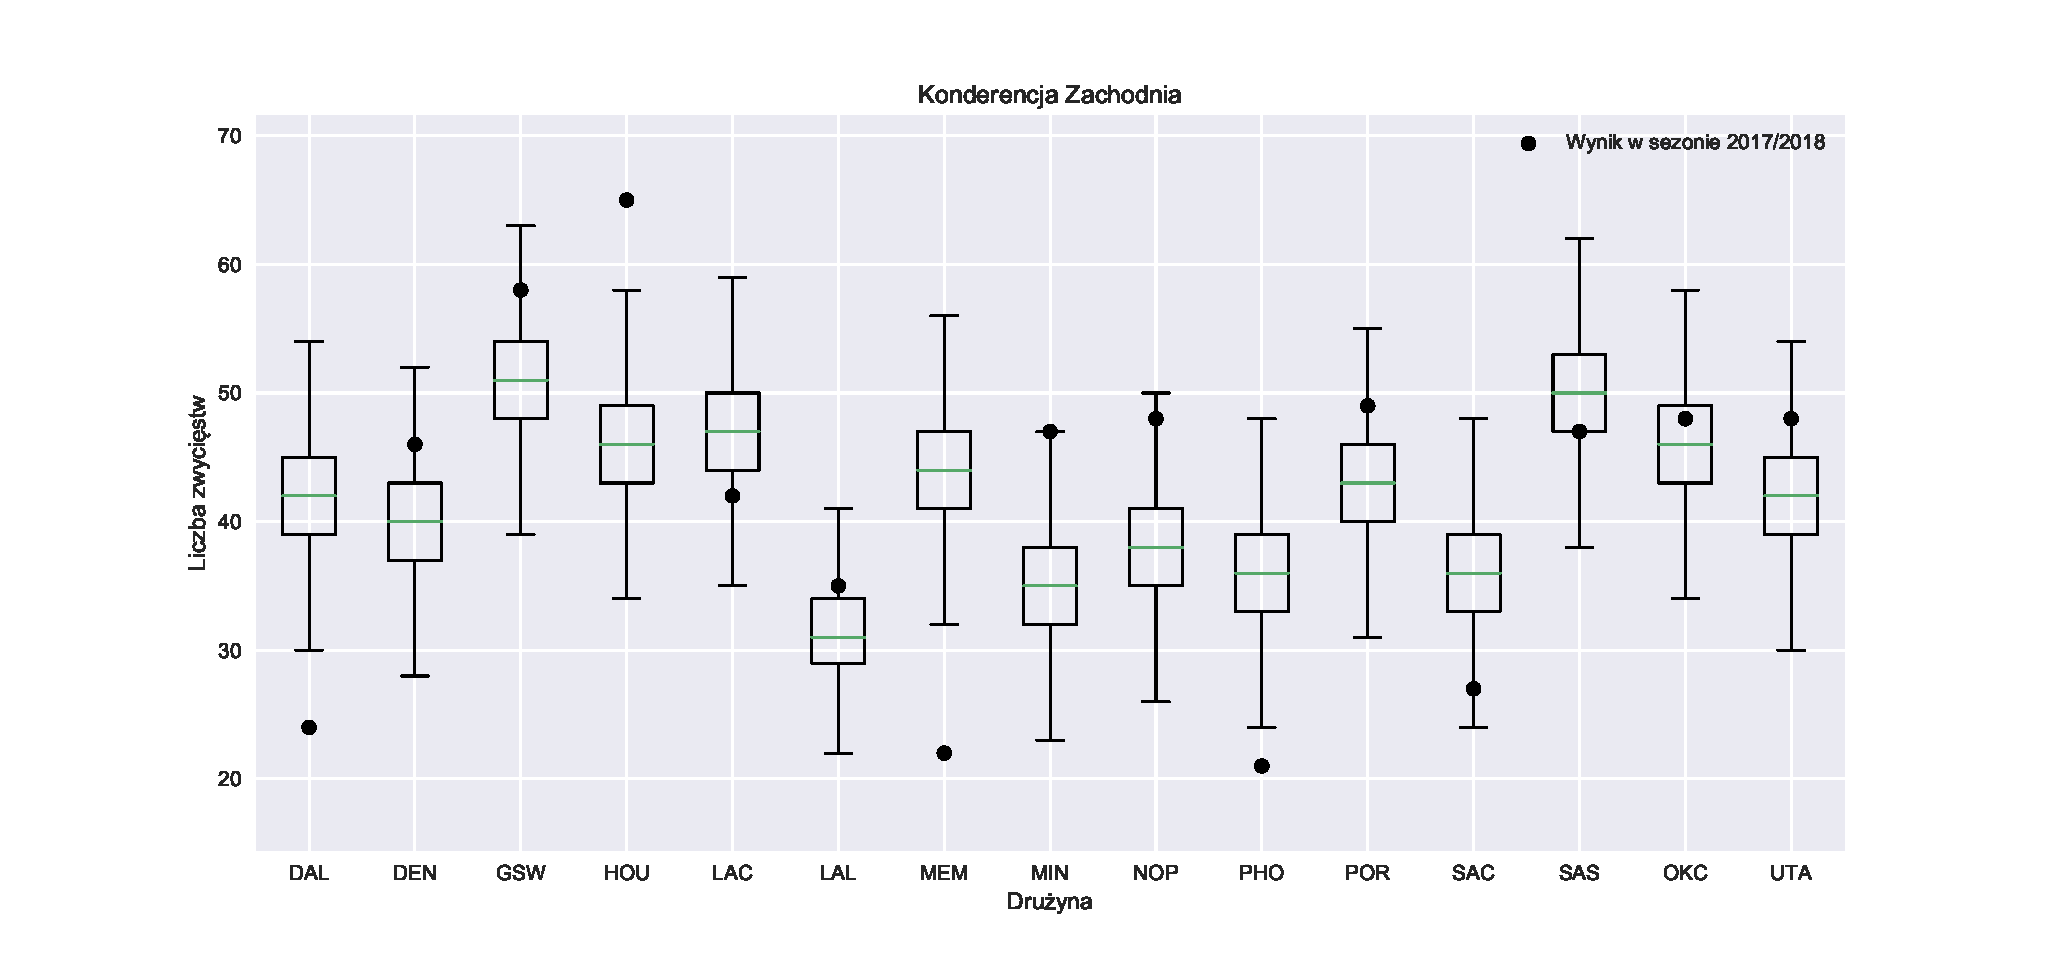
\includegraphics[width=22cm]{m1_dla17_5lat_waga1_box_zachod.pdf}
	\caption{Wykres pudełkowy wyników symulacji sezonu przy użyciu modelu I, na podstawie danych z 5 lat i wadze $x=1$, Konferencja Zachodnia}
	\label{m1_5lat_waga1_zachod_17}
	\centering
\end{figure}

\begin{figure}[t]
	\hspace*{-3cm}  
	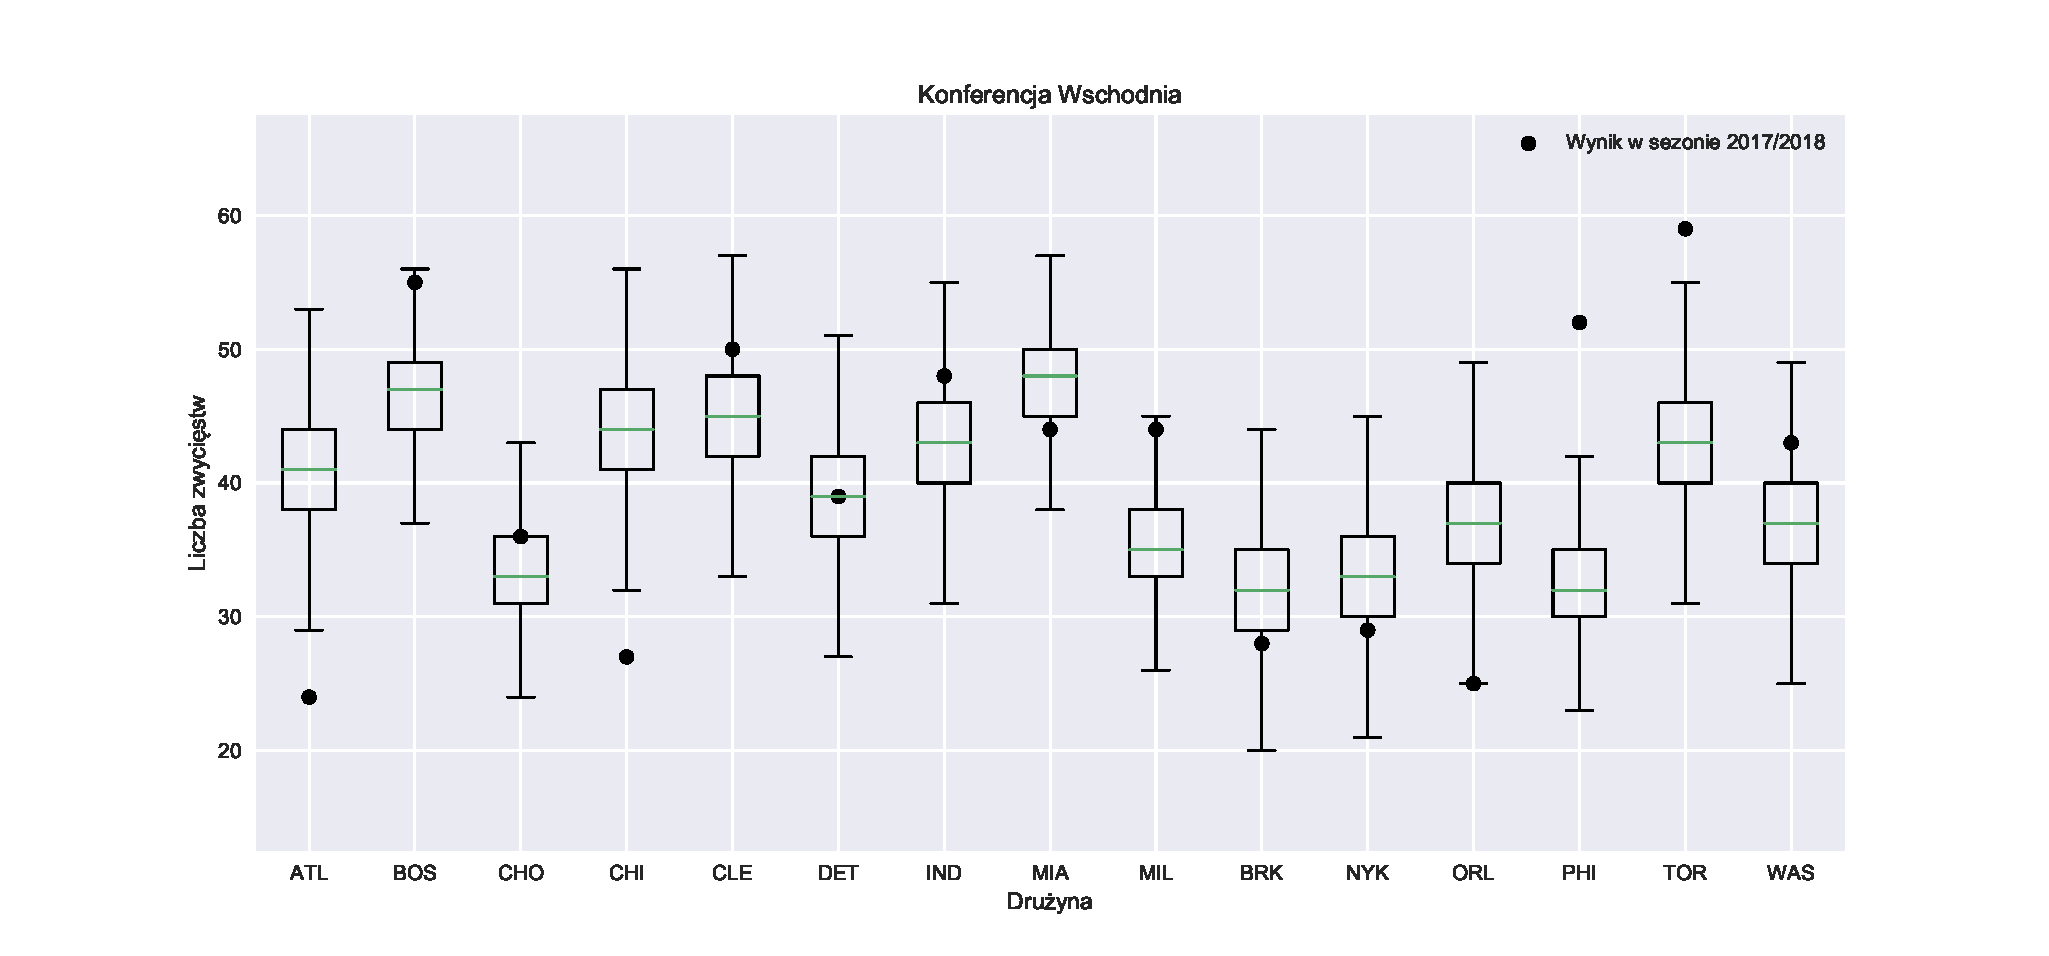
\includegraphics[width=22cm]{m2_dla17_10lat_waga05_box_wschod.pdf}
	\caption{Wykres pudełkowy wyników symulacji sezonu przy użyciu modelu II, na podstawie danych z 10 lat i wadze $x=0.5$, Konferencja Wschodnia}
	\label{m2_10lat_waga05_wschod_17}
	\centering
\end{figure}

\begin{figure}[t]
	\hspace*{-3cm}  
	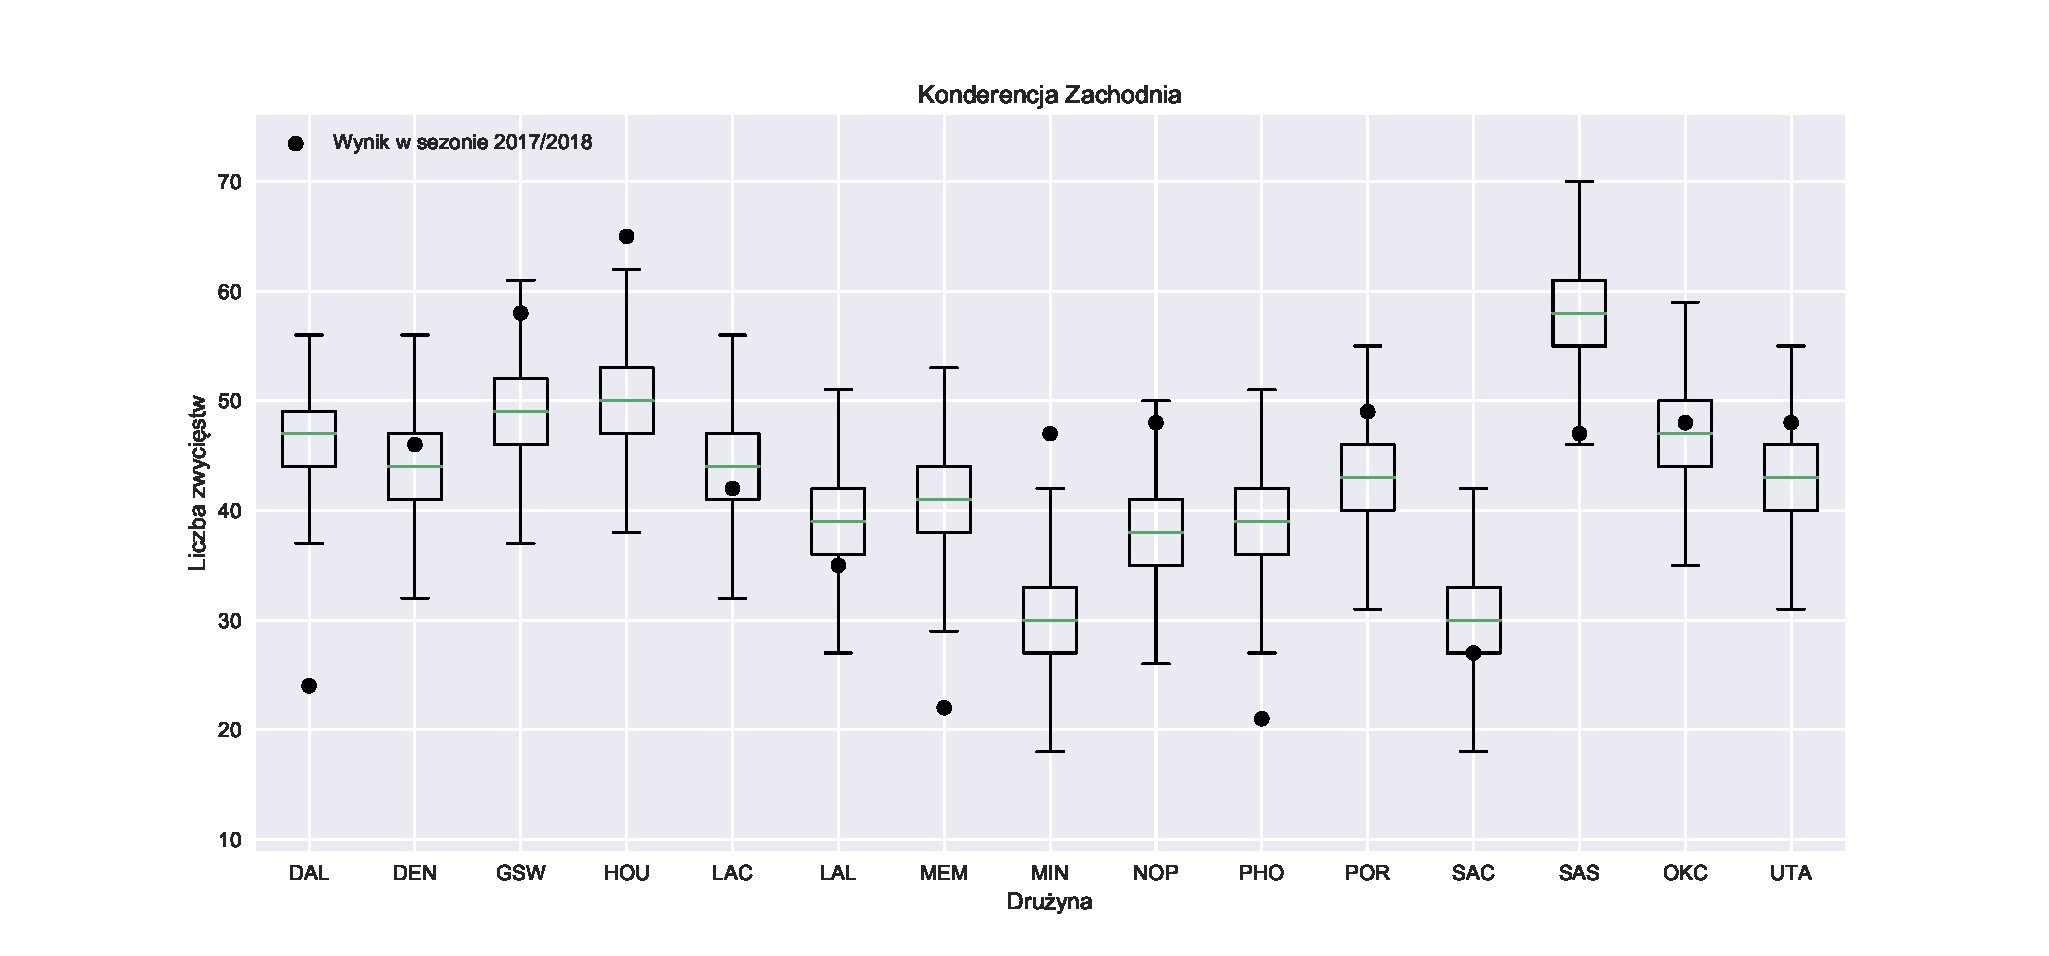
\includegraphics[width=22cm]{m2_dla17_10lat_waga05_box_zachod.pdf}
	\caption{Wykres pudełkowy wyników symulacji sezonu przy użyciu modelu II, na podstawie danych z 10 lat i wadze $x=0.5$, Konferencja Wschodnia}
	\label{m2_10lat_waga05_zachod_17}
	\centering
\end{figure}
Analizując wykresy pudełkowe można zauważyć, że:
\begin{itemize}
	\item liczba dopasowań bardzo dobrych, czyli leżących w przedziale $[Q_1,Q_3]$ jest lepsza dla modelu II i wynosi 6, podczas gdy dla modelu I wartość ta jest równa 5. Większość drużyn osiąga wyniki na podobnym poziomie.
	\item liczba wartości odstających, leżących poza przedziałem $[Q_1-1.5IQR,Q_3+1.5IQR]$ jest większa dla modelu II, jest równa 8, gdzie dla modelu I równa się ona 7.
\end{itemize}
Patrząc na te wyniki nie można jednoznacznie odrzucić jednego modelu na korzyść drugiego, dlatego do wybrania najlepszego z nich dokonano również analizy rozgrywek pucharowych. Ponownie analizując tabelę z wartościami $G$ można zauważyć, że w dla rozgrywek 2017/2018 symulacje były bardziej trafne. Wyraźnie większa dokładność w przypadku późniejszego sezonu wynika z faktu, że od kilku lat obserwuje się te same drużyny w czołówce ligi. Przed 2014 rokiem równowaga została zachwiana przez przejście jednego z najlepszych graczy ligi, LeBrona Jamesa z Miami Heat do Cleveland Cavaliers, jak i rozpowszechnienie przez Golden State Warriors systemu szybkiej gry opartej na rzutach z dystansu. W trakcie lata 2018 roku LeBron ponownie zmienił klub, tym razem na Los Angeles Lakers, co może mieć znaczący wpływ na jakość predykcji trwającego sezonu (drużyny, w których gra pojawiają się w Finałach NBA nieprzerwanie od 2010 roku). 

\subsection{Wyniki symulacji dla fazy playoff}
Dla wybranych w poprzedniej części modeli i parametrów przeprowadzona została symulacja rozgrywek pucharowych, korzystając z algorytmów zdefiniowanych w rozdziale \ref{modele_palyoff}. W tabeli \ref{tabela_playoffs2018} porównano przewidziane na ich podstawie serie wraz z rzeczywistym przebiegiem rozgrywek w 2018 roku. Podczas symulowania tej fazy trzymano się zasady, wedle której drużyna z lepszym bilansem wypisana jest jako pierwsza. 

\begin{table}[]
	\centering
	\begin{tabular}{ll}

	\begin{tabular}{|c|c|c|}
	\hline
	\multicolumn{3}{|c|}{\textbf{Prognozy dla wybranego Modelu I}} \\\hline
	\multicolumn{3}{|c|}{} \\\hline	
	\textbf{Model IV}& \textbf{Model V} &\textbf{Rzeczywistość}\\\hline	
	
	\multicolumn{3}{|c|}{} \\\hline	
	\multicolumn{3}{|c|}{\textbf{Eastern Conference First Round}} \\\hline
	CLE-WAS&TOR-CLE  &TOR-WAS\\\hline
	MIA-BOS&WAS-CHI &CLE-IND\\\hline
	ATL-CHI&ATL-BOS &PHI-MIA\\\hline
	TOR-IND&BRK-MIA &BOS-MIL\\\hline
	\multicolumn{3}{|c|}{} \\\hline
	
	\multicolumn{3}{|c|}{\textbf{Western Conference First Round}} \\\hline
	GSW-DAL&NOP-OKC &HOU-MIN\\\hline
	HOU-OKC&UTA-LAC &OKC-UTA\\\hline
	LAC-MEM&POR-SAS &POR-NOP\\\hline
	SAS-NOP&GSW-HOU &GSW-SAS\\\hline
	\multicolumn{3}{|c|}{} \\\hline
	
	\multicolumn{3}{|c|}{\textbf{Eastern Conference Semifinals}} \\\hline
	CLE-MIA&IND-TOR &TOR-CLE\\\hline
	TOR-ATL&CHO-ATL &BOS-PHI\\\hline
	\multicolumn{3}{|c|}{} \\\hline
	
	\multicolumn{3}{|c|}{\textbf{Western Conference Semifinals}} \\\hline
	GSW-HOU&SAS-GSW &HOU-UTA\\\hline
	SAS-LAC&UTA-MEM &GSW-NOP\\\hline
	\multicolumn{3}{|c|}{} \\\hline
	
	\multicolumn{3}{|c|}{\textbf{Eastern Conference Finals}} \\\hline
	CLE-TOR&CLE-CHI &BOS-CLE\\\hline
	\multicolumn{3}{|c|}{} \\\hline
	
	\multicolumn{3}{|c|}{\textbf{Western Conference Finals}} \\\hline
	GSW-SAS&GSW-SAS &HOU-GSW\\\hline
	\multicolumn{3}{|c|}{} \\\hline
	
	\multicolumn{3}{|c|}{\textbf{Finals}} \\\hline
	GSW-TOR& GSW-TOR &GSW-CLE\\\hline
	\multicolumn{3}{|c|}{} \\\hline
	
	\multicolumn{3}{|c|}{\textbf{Zwycięzca}} \\\hline
	GSW&  GSW&GSW\\\hline
	\end{tabular}

	\begin{tabular}{ |c|c|c|  }
		\hline
		\multicolumn{3}{|c|}{\textbf{Prognozy dla wybranego Modelu II}} \\\hline
		\multicolumn{3}{|c|}{} \\\hline	
		\textbf{Model IV}& \textbf{Model V} &\textbf{Rzeczywistość}\\\hline	
		
		\multicolumn{3}{|c|}{} \\\hline	
		\multicolumn{3}{|c|}{\textbf{Eastern Conference First Round}} \\\hline
		MIA-WAS& CHI-CLE &TOR-WAS\\\hline
		BOS-CLE&BOS-IND &CLE-IND\\\hline
		CHI-TOR&MIA-TOR &PHI-MIA\\\hline
		ATL-IND&ATL-BRK &BOS-MIL\\\hline
		\multicolumn{3}{|c|}{} \\\hline
		
		\multicolumn{3}{|c|}{\textbf{Western Conference First Round}} \\\hline
		SAS-POR&SAS-DAL &HOU-MIN\\\hline
		LAC-HOU&GSW-POR &OKC-UTA\\\hline
		OKC-MEM& HOU-NOP&POR-NOP\\\hline
		GSW-NOP& LAC-OKC&GSW-SAS\\\hline
		\multicolumn{3}{|c|}{} \\\hline
		
		\multicolumn{3}{|c|}{\textbf{Eastern Conference Semifinals}} \\\hline
		MIA-BOS& MIA-CLE&TOR-CLE\\\hline
		ATL-CHI& ATL-BOS&BOS-PHI\\\hline
		\multicolumn{3}{|c|}{} \\\hline
		
		\multicolumn{3}{|c|}{\textbf{Western Conference Semifinals}} \\\hline
		SAS-LAC& SAS-LAC&HOU-UTA\\\hline
		OKC-GSW& OKC-GSW&GSW-NOP\\\hline
		\multicolumn{3}{|c|}{} \\\hline
		
		\multicolumn{3}{|c|}{\textbf{Eastern Conference Finals}} \\\hline
		MIA-CHI& MIA-CHI&BOS-CLE\\\hline
		\multicolumn{3}{|c|}{} \\\hline
		
		\multicolumn{3}{|c|}{\textbf{Western Conference Finals}} \\\hline
		SAS-GSW& SAS-GSW&HOU-GSW\\\hline
		\multicolumn{3}{|c|}{} \\\hline
		
		\multicolumn{3}{|c|}{\textbf{Finals}} \\\hline
		MIA-SAS&  MIA-SAS&GSW-CLE\\\hline
		\multicolumn{3}{|c|}{} \\\hline
		
		\multicolumn{3}{|c|}{\textbf{Zwycięzca}} \\\hline
		SAS&  SAS&GSW\\\hline
	\end{tabular}
\end{tabular}
	\caption{Przebieg serii playoff w symulacjach dla 2018 roku}\label{tabela_playoffs2018}
\end{table}

Po przeanalizowaniu wyników okazało się, że prognozy wynikające z modelu V są całkowicie nietrafne --- kombinacje zespołów w następnych rundach nie pokrywają się z poprzednimi. Podczas predykcji rundy pierwszej wskazał on poprawnie 12 z 16 drużyn (wyniki dla sezonu symulowanego modelem I), z czego dla Konferencji Wschodniej błędnie wyznaczone były aż 3 z 5 organizacji. Dla porównania, podczas szacowania przebiegu modelu II pomylił się w przypadku 5 drużyn. Przy dalszych rozważaniach model ten został odrzucony --- pomimo porównywalnej dokładności z modelem IV (takie same liczby poprawnie wytypowanych drużyn) jego ogromną wadą jest brak konsekwentności, czego najlepszym przykładem jest przewidziana seria Charlotte-Atlanta w finałach Konferencji Wschodniej (Charlotte nie zostało wytypowane do gry w pierwszej rundzie).
 
Po odrzuceniu jednej z metod predykcji fazy pucharowej zbadano przebieg przewidywanych rozgrywek w oparciu o model IV wykorzystujący dane o sezonach zasadniczych generowanych przy wykorzystaniu modeli dobranych we wcześniejszych rozważaniach. Obydwa modele sprawdzały się podobnie w przypadku rundy pierwszej, jednak od rundy drugiej szacunki zaczęły być znacznie bardziej dokładne:
\begin{itemize}
	\item w przypadku modelu I do Półfinałów Konferencji Wschodniej zakwalifikowały się 2 z 4 drużyn, dla modelu II natomiast nie przeszła żadna z rzeczywistych drużyn,
	\item dla Półfinałów Konferencji Zachodniej model I wygrał ponownie,  przewidując słusznie 2 drużyny, przy 1 dla konkurenta,
	\item w Finałach Konferencji Model I jeszcze raz okazał się lepszy, za każdym razem dobrze przewidując przynajmniej jednego finalistę, podczas gdy drugi z systemów był skuteczny tylko dla 1 z 4 zespołów,
	\item model I słusznie przewidział zwycięzcę całej ligi.
\end{itemize}
Pomimo faktu, że model IV nie przewidział pojawienia się w tej części sezonu zespołów z Milwaukee, Filadelfii, Minnesoty i Utah, był w stanie stosunkowo dobrze wytypować dalsze etapy rozgrywek, dlatego też zostanie wykorzystany w dalszych pracach.

\subsection{Symulacja sezonu 2018/2019}
W poprzedniej części pracy udowodniono, że przewidywania najtrafniejsze będą, jeżeli sezon zasadniczy symulowany będzie przy pomocy modelu I, danych z ostatnich 5 lat, i wagi $x=1$. W przypadku fazy pucharowej do predykcji rozgrywek playoff wykorzystany zostanie model IV. Wyniki symulacji można odczytać z rysunków \ref{m1_dla18_5lat_waga1_box_wschod} i \ref{m1_dla18_5lat_waga1_box_zachod}, jak i tabeli \ref{tabela_symulacja_2018}.
\begin{figure}[t]
	\hspace*{-3cm}  
	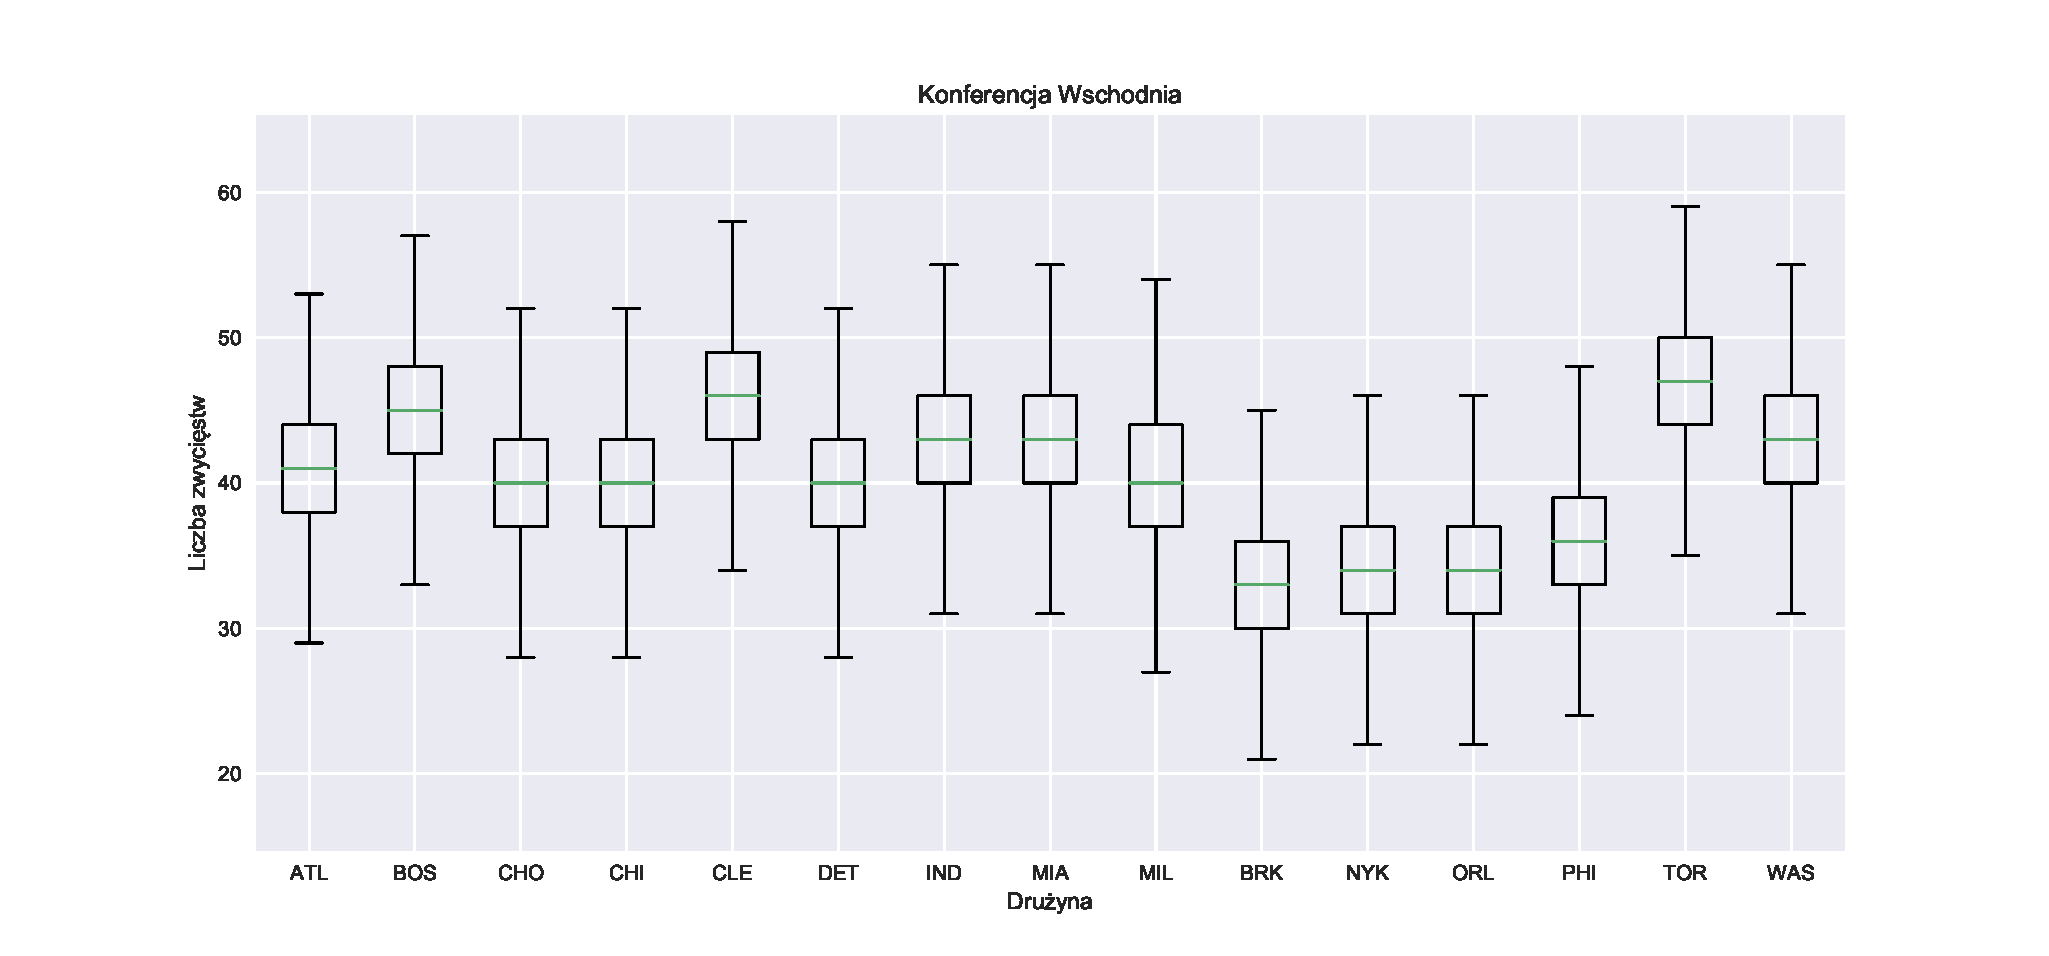
\includegraphics[width=22cm]{m1_dla18_5lat_waga1_box_wschod.pdf}
	\caption{Szacowane wyniki w sezonie 2018/2019}
	\label{m1_dla18_5lat_waga1_box_wschod}
	\centering
\end{figure}
\begin{figure}[t]
	\hspace*{-3cm}  
	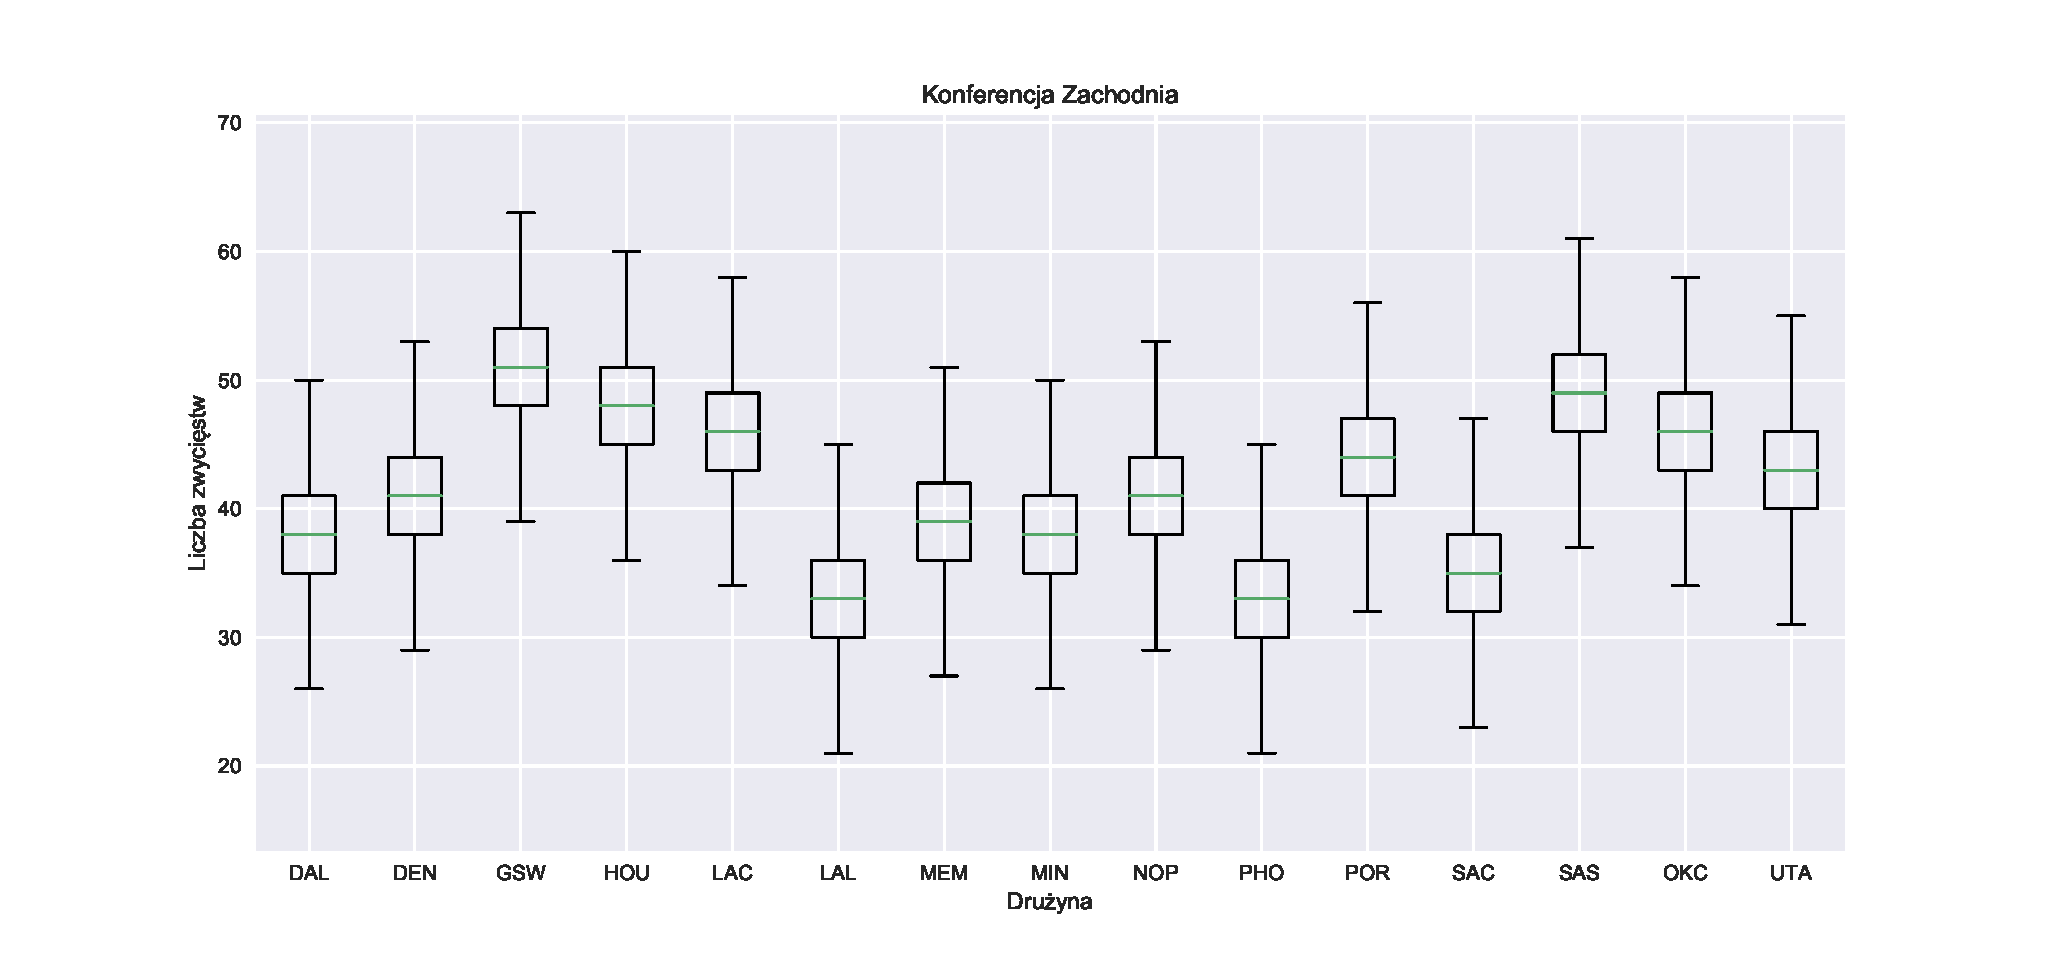
\includegraphics[width=22cm]{m1_dla18_5lat_waga1_box_zachod.pdf}
	\caption{Szacowane wyniki w sezonie 2018/2019}
	\label{m1_dla18_5lat_waga1_box_zachod}
	\centering
\end{figure}
\begin{table}[]
	\centering
	\begin{tabular}{ll}
	\begin{tabular}{|c|c|c|}
		\hline
		\multicolumn{3}{|c|}{\textbf{Prognozy sezonu zasadniczego}} \\\hline
		&\multicolumn{2}{|c|}{Liczba zwycięstw} \\\hline	
		\textbf{Drużyna}      & \textbf{Model I} & \textbf{ESPN}\\ \hline
		Atlanta Hawks & 41 & 22\\ \hline
		Boston Celtics & 45 & 58\\ \hline
		Brooklyn Nets & 33 & 32\\ \hline
		Charlotte Hornets & 40 & 35\\ \hline
		Chicago Bulls & 40 & 28\\ \hline	
		Cleveland Cavaliers & 46 & 31\\ \hline
		Dallas Mavericks & 38& 33\\ \hline	
		Denver Nuggets & 41 & 47\\ \hline
		Detroit Pistons & 40 & 44\\ \hline
		Golden State Warriors & 51 & 58\\ \hline
		Houston Rockets & 48 & 57\\\hline
		Indiana Pacers & 43 & 47\\\hline
		Los Angeles Clippers & 46 &35\\ \hline
		Los Angeles Lakers & 33 & 46\\ \hline
		Memphis Grizzlies & 39 &33\\ \hline
		Miami Heat & 43 & 47 \\\hline
		Milwaukee Bucks & 40 & 47\\ \hline
		Minnesota Timberwolves & 38 & 45\\ \hline
		New Orleans Pelicans & 41  &45\\ \hline
		New York Knicks & 34 & 28\\ \hline
		Oklahoma City Thunder & 46 & 49\\ \hline
		Orlando Magic & 35 & 30\\ \hline
		Philadelphia 76ers & 36 & 53\\ \hline
		Phoenix Suns & 36 &27\\\hline
		Portland Trail Blazers & 44& 43\\ \hline	
		Sacramento Kings & 35 &24\\ \hline
		San Antonio Spurs & 49 &44\\ \hline
		Toronto Raptors & 47 & 55\\ \hline
		Utah Jazz & 43 & 49\\\hline
		Washington Wizards & 43 & 44\\ \hline
	\end{tabular}

	\begin{tabular}{|c|c|}
		\hline
		\multicolumn{2}{|c|}{\textbf{Prognozy fazy pucharowej}} \\\hline
		\multicolumn{2}{|c|}{} \\\hline	
		\textbf{Wschód}& \textbf{Zachód}\\\hline	
		
		\multicolumn{2}{|c|}{} \\\hline	
		\multicolumn{2}{|c|}{\textbf{First Round}} \\\hline
		TOR-CHO&GSW-NOP \\\hline
		IND-WAS&LAC-OKC\\\hline
		BOS-MIA&HOU-POR\\\hline
		CLE-ATL&SAS-UTA\\\hline
		\multicolumn{2}{|c|}{} \\\hline
		
		\multicolumn{2}{|c|}{\textbf{Conference Semifinals}} \\\hline
		TOR-IND&GSW-LAC \\\hline
		CLE-BOS&SAS-HOU \\\hline
		\multicolumn{2}{|c|}{} \\\hline

		\multicolumn{2}{|c|}{\textbf{Conference Finals}} \\\hline
		TOR-CLE&GSW-SAS \\\hline
		\multicolumn{2}{|c|}{} \\\hline
		
		\multicolumn{2}{|c|}{\textbf{Finals}} \\\hline
		\multicolumn{2}{|c|}{GSW-TOR} \\\hline
		\multicolumn{2}{|c|}{} \\\hline
		
		\multicolumn{2}{|c|}{\textbf{Zwycięzca}} \\\hline
		\multicolumn{2}{|c|}{GSW} \\\hline
	\end{tabular}
\end{tabular}
	\caption{Wyniki symulacji sezonu 2018/2019}\label{tabela_symulacja_2018}	
\end{table}
Porównując rezultaty przeprowadzonych prognoz z poprzednimi symulacjami można zauważyć pewną tendencję --- zaproponowane w tej pracy modele nie zakładają sytuacji, w której zespół wchodzi w stan przebudowy i zaczyna przegrywać. Z tego powodu oszacowane liczby wygranych można uznać za bardzo optymistyczne, ponieważ wiadome jest, że zespoły takie jak Brooklyn Nets, Phoenix Suns, Atlanta Hawks, czy New York Knicks najprawdopodobniej nie osiągną przewidywanych wyników. Podobnie sytuacja ma się w fazie pucharowej, gdzie z powodu nagłego osłabienia Cleveland zespoły, które do tej pory w cieniu wzmacniały swoje składy, mają realną szansę na walkę o najwyższe cele. Po zestawieniu wyników modelu I z przewidywaniami ESPN \cite{espn} można zauważyć, że rezultaty zaproponowane w obu modelach pokrywają się z nielicznymi wyjątkami --- są to kluby, które znacząco wzmocniły się tego lata lub weszły w przebudowę. 

\chapter{Wnioski}
Podczas symulowania rozgrywek i porównywania ich wyników z rzeczywistymi okazało się, że w wielu przypadkach zasugerowane modele nie oddają dobrze przebiegu sezonu. Należy pamiętać, że zawodnicy z czasem przestają grać na wysokim poziomie, zmieniają kluby, łapią kontuzje, czy nawet przechodzą na emerytury. Przykładem organizacji, która pomimo regresu w ostatnich sezonach, jest wysoko notowana we wszystkich symulacjach są San Antonio Spurs. Trzon tego zespołu od kilkunastu lat był taki sam i grał na niezwykle wysokim poziomie, zdobywając wielokrotne mistrzostwa od 2000 roku. Jednak ostatnie lata przyniosły spadek formy wielu gwiazd związany z wiekiem, co doprowadziło do zakończenia ich karier. Wszystkie modele klasyfikują tę drużynę bardzo wysoko ze względu na zeszłe dokonania, co prowadzi do mało prawdopodobnych wyników predykcji. Kolejnym niemożliwym do przewidzenia czynnikiem jest decyzja zarządu klubu o celowym przegrywaniu --- skutkiem tego są ich bardzo niskie wyniki i podwyższone wygrane innych zespołów. Wysoce prawdopodobne jest, że zaproponowane w tej pracy modele dałyby bardziej precyzyjne wyniki, gdyby żadna drużyna nie decydowała się na przebudowę poprzez odpuszczanie meczów. Osobną kwestią jest również etap, w którym zespoły rozwijające młodzież zaczynają nagle wygrywać, ponieważ niejednokrotnie po wielu słabych latach z zaskoczenia osiągały wysokie rezultaty (na przykład Philaledphia 76ers, po kilku sezonach ciągłego przegrywania zajęli niespodziewanie trzecie miejsce na Wschodzie). Modele symulujące rozgrywki pucharowe również miały te same problemy, jednak w większości przypadków skutecznie udawało im się przewidywać kształt Finałów Konferencji i wytypować zwycięzców ligi. Okazało się, że najdokładniejsze były dla stabilnego sezonu 2017/2018, można więc założyć, że wszystkie algorytmy działają najlepiej dla stabilnej ligi, w której drużyny grają stale na tym samym poziomie.

{\backmatter \chapter{Podsumowanie}}
W niniejszej pracy inżynierskiej zaproponowano kilka modeli umożliwiających symulowanie rozgrywek NBA w oparciu o dane zawierające wyniki z zeszłych sezonów. Wszystkie modele przetestowano dla różnych okresów zbierania danych, wag premiujących kolejne lata, jak i sezonu, dla którego dokonano symulacji. Wybrano w ten sposób najlepszy system do predykcji wyników wybranego sezonu. Niestety, okazało się, że zaproponowane metody nie oddają w pełni trendów panujących obecnie w NBA, jak i nie działają najlepiej w przypadku nagłej poprawy gry przez słabe do tej pory zespoły. Dokonano porównania wyników zaproponowanego modelu z prognozami ESPN i zauważono, że w większej części tendencje w nich są podobne. W trakcie badania skuteczności modeli testowano normalność rozkładu zwycięstw każdej z drużyn w próbie bootstrap, jednak we wszystkich testach hipotezy te zostały odrzucone. Dalsze rozważania na ten temat spowodowały wysnucie hipotezy, wedle której zwycięstwa te pochodzą z mieszanego rozkładu dwumianowego, jednak udowodnienie tego było niemożliwe. Uzyskawszy nie najlepsze wyniki takiego podejścia do szacowania rezultatów sezonu warte rozważenia jest stworzenie modelu opierającego się na statystykach zawodników grających w poszczególnych klubach i ich wpływie na grę.

{\backmatter \chapter{Dodatek}}
Ze względu na dużą ilość tabel z danymi i wygenerowanych dla nich wykresów, wszystkie dodatki zostały zawarte na płycie dołączonej do pracy.
%Dodatek w pracach matematycznych również nie jest wymagany. Można w nim przedstawić np. jakiś dłuższy dowód, który z pewnych przyczyn pominęliśmy we właściwej części pracy lub (np. w przypadku prac statystycznych) umieścić dane, które analizowaliśmy.

%%%%%%%%%%%%%%%%%%%%%%%%%%%%%%%%%%%%%%%%%%%%%%%%%%%%%%%%%
% BIBLIOGRAFIA
% W tworzeniu bibliografii najlepiej korzystać z BibTex'a, 
% który jest częścią systemu Tex. W naszym przypadku funkcję 
% przechowalni literatury, do której się odwołujemy, pełni 
% plik bibliografia.bib. Nie musimy ręcznie dodawać nowych 
% pozycji do bibliografii. Możemy wejść np. na stronę 
% https://mathscinet.ams.org/mathscinet/index.html, 
% znaleźć odpowiednią pozycję, wybrać ją, a następnie zmienić 
% 'Select alternative format' na BibTeX, skopiować uzyskany 
% tekst, wkleić do pliku bibliografia.bib i skompilować. 
% Gotowe informacje do pliku bibliografia.bib można znaleźć 
% także na https://arxiv.org - gdy znajdziemy interesującą nas 
% pracę, szukamy 'References & Citations' i klikamy 'NASA ADS', 
% a potem 'Bibtex entry for this abstract' 
% i postępujemy tak jak wcześniej.
%%%%%%%%%%%%%%%%%%%%%%%%%%%%%%%%%%%%%%%%%%%%%%%%%%%%%%%%%
\newpage
% w nawiasie klamrowym wpisujemy nazwę pliku z bibliografią w formacie .bib
%\bibliografia{bibliografia} 

\begin{thebibliography}{9}	
	\bibitem{efron1}
	\emph{B. Efron: Bootstrap methods: another look at the jackknife. The Annals of Statistics 1979, Vol. 7, No. 1, 1--26 }
	
	\bibitem{efron2}
	\emph{B. Efron: The jackknife, the bootstrap, and other resampling plans. SIAM, 1982}
	
	\bibitem{espn}
	\emph{ESPN: Summer Forecast: East standings, West standings for 2018-19, 14 sierpnia 2018, [dostęp: 9 grudnia 2018], http://www.espn.com/nba/story/\_/id/24365036/nba-standings-predictions-espn-summer-forecast}
	
	\bibitem{monte}
	\emph{M. Haugh: Generating Random Variables and Stochastic Processes, Columbia University, 2017, [dostęp: 4 grudnia 2018], <http://www.columbia.edu/~mh2078/MonteCarlo/MCS\_Generate\_RVars.pdf>}
	
	\bibitem{koronacki}
	\emph{J. Koronacki, J. Mielniczuk: Statystyka dla studentów kierunków technicznych i przyrodniczych, Wydawnictwo Naukowo-Techniczne, Warszawa, 2009}
	
	\bibitem{magiera}
	\emph{R. Magiera: Modele i metody statystyki matematycznej. Część II. Wnioskowanie statystyczne. Wydanie drugie rozszerzone, Oficyna Wydawnicza GiS, Wrocław, 2007}
	
	\bibitem{graphicalNBA}
	\emph{M. Oh, S. Keshri, G. Iyengar: Graphical Model for Baskeball Match Simulation, Sloan Sports Analytics Conference, 2015 [dostęp: 1 grudnia 2018], <http://www.sloansportsconference.com/wp-content/uploads/2015/02/SSAC15-RP-Finalist-Graphical-model-for-basketball-match-simulation.pdf>}
	
	\bibitem{replayNBA}
	\emph{N. Sandholtz, L. Bornn: Replaying the NBA, Sloan Sports Analytics Conference, 2018 [dostęp: 5 grudnia 2018], <http://www.lukebornn.com/papers/sandholtz\_ssac\_2018.pdf>}
		
	\bibitem{bootstrap2}
	\emph{C. Shalizi: The Bootstrap, 3 luty 2011, [dostęp: 3 grudnia 2018], <https://www.stat.cmu.edu/~cshalizi/402/lectures/08-bootstrap/lecture-08.pdf>}
	
	\bibitem{bootstrap1}
	\emph{K. Singh, M. Xie: Bootstrap: A Statistical Method, Rutgers University, [dostęp: 16 grudnia 2018], <http://www.stat.rutgers.edu/home/mxie/stat586/handout/Bootstrap1.pdf>}
		
	\bibitem{dane}
	\emph{Basketball-Reference.com: Basketball Statistics and History, <https://www.basketball-reference.com/>}
		
	\bibitem{playoffs}
	\emph{DevianArt, [dostęp: 9 grudnia 2018],\\ <https://pre00.deviantart.net/d550/th/pre/i/2017/089/a/0/nba\_playoff\_bracket\_by\_nbaplayoffs-db410wn.jpg>}
	
	\bibitem{mapa}
	\emph{How many teams are in each conference in the NBA?, Maps of World, 9 lipca 2017, [dostęp: 16 grudnia 2018], <https://www.mapsofworld.com/answers/united-states/many-teams-conference-nba/>}
	
	\bibitem{houston}
	\emph{Moreyball: The Houston Rockets and Analytics, Harvard Business School, 5 kwietnia 2018, [dostęp: 6 grudnia 2018] <https://digit.hbs.org/submission/moreyball-the-houston-rockets-and-analytics/>}
	
	\bibitem{history}
	\emph{NBA History, NBA Hoops Online, [dostęp: 14 listopada 2018], <https://nbahoopsonline.com/History/>}

\end{thebibliography}


\end{document}

